% !Mode:: "TeX:UTF-8"
% !Mode:: "TeX:UTF-8"
% !TEX root = tjumain.tex


\baselineskip=20pt

%%%% 第一章:绪论 %%%%%
\chapter{绪论}
\section{引言}

虚拟化是一个在复杂计算系统和体系结构中被广泛应用的技术。今天业界所认为的大部分云系统都是在数据中心强大的服务器上的虚拟机中相互隔离运行的大量应用程序。这些应用的虚拟化特性十分灵活,可以抽象出特定的硬件模式,因此许多软件可以直接运行在许多系统中。

虚拟化技术的研究来源于对计算机系统性能和效率的不断追求,它可以解决传统物理系统存在的资源浪费、管理复杂、难以扩展等问题。

RISC -V 作为新兴的指令集架构,它的虚拟化技术仍然处于初始阶段,因此研究 RISC -V 的虚拟化技术是很有意义的,它可以促进 RISC -V 处理器架构在服务器领域的发展与应用,因为服务器需要一个稳定的虚拟化软件生态环境;也可以帮助增加 RISC -V 处理器架构的兼容性和灵活性,通过 RISC -V hypervisor 可以支持多种类型的操作系统,例如 Linux、Windows 以及 FreeBSD 等;除此之外,RISC -V hypervisor 可以利用 RISC -V 处理器架构的开放性和可扩展性,实现更高效和更安全的虚拟化机制,例如使用硬件辅助或者微内核技术。除此之外,较小规模的虚拟化也被广泛应用于隔离嵌入式平台上的应用程序,一个例子是 Siemens Jailhouse\cite{sinitsyn2015jailhouse},它是开源的且可以公开获取。

本次课题来源于我个人对 RISC-V 的兴趣与长期关注,以及对于虚拟化技术的兴趣。因此为了检验 RISC-V 虚拟化技术的成熟度与 Rust 语言编写 hypervisor 的能力,本次工作历时数个月的时间,从零开始编写了两版 hypervisor,hypocaust 以及 hypocaust-2,hypocaust 是使用 Rust 编写的第一版 RISC-V Type-1 hypervisor,使用了 S mode 陷入与模拟技术,目前可以启动一个小型的带文件系统的操作系统;hypocaust-2 是使用 Rust 编写的第二版 RISC-V Type-1 hypervisor,使用了 RISC-V Hypervisor Extension 硬件辅助虚拟化技术,目前已经可以启动 rCore-Tutorial-v3,RT-Thread 以及 Linux mainline。
除此之外,本次工作也在 2023 年 3 月 26 日北京召开的第十届开源操作系统年度技术会议中做了邀请报告,介绍了 RISC-V 虚拟化技术以及本次工作的实现细节。除此之外,本次课题所衍生出的相关工作也在第三届全国大学生操作系统大赛的功能赛道中作为赛题出现。

本工作的主要贡献有:
\begin{itemize}
    \item 使用 Rust 语言从零开始编写了两版 RISC-V hypervisor。
    \item 通过实践证明了 RISC-V 虚拟化技术的可行性与成熟度。
    \item 总结了从零开始编写一个可以启动 Linux 的小型 Type-1 hypervisor 的过程与经验。
\end{itemize}

\section{研究背景与意义}
Hypervisor 是一种虚拟化技术,它可以在一台物理计算机上运行多个虚拟机。Hypervisor 的发展历史可以追溯到 1960 年代中期,当时大型机统治着计算机市场。在那个时候,虚拟化技术被用于将大型机的计算能力分配给多个用户。
第一代 hypervisor 诞生于 20 世纪 60 年代,也称为“裸机式与硬件式”,是最初的虚拟化技术,启动时直接在物理硬件上运行,它没有底层操作系统,而是直接运行虚拟机,通过直接访问硬件资源提供更高的效率。

第二代 hypervisor,也称为 "Hosted 模式",意味着 hypervisor 运行在一个完整的操作系统上。这种方法在 PC 和服务器领域越来越流行,因为它适用于更广泛的硬件和操作系统,并且更容易实现,这一代的 hypervisor 可以在主机操作系统(例如 Linux、Windows)上运行和创建虚拟机。

第三代 hypervisor,也称为“半虚拟化”和“Para-virtualization”,它在第二代 hypervisor 的基础上进一步发展。它的特点是通过修改虚拟机中的操作系统来驱动底层硬件。这种方法可以减少 hypervisor 的负担,并提高系统的性能。最初的例子包括 Xen,后来 VMware ESX Server 也支持这种技术。

第四代 hypervisor 是在第二代和第三代 hypervisor 的基础上发展而来,它在物理硬件和虚拟机之间增加了一层硬件辅助,从而更好的控制和保护虚拟化的环境。这种 hypervisor 通常是由处理器厂商(如 Intel 和 AMD)提供的,如 Intel VT 和 AMD-V。虚拟化软件可以利用这些硬件特性来实现高效的虚拟化。举例来说,VMware vSphere 和 Microsoft Hyper-V 就是基于此的虚拟化环境。

如今学术界与工业界对于虚拟化技术的研究大多集中在 x86、ARM 等主流指令集架构上,而对于新兴架构 RISC-V 的虚拟化技术研究较少,因此本次课题专注于对于 RISC-V 虚拟化技术的研究,希望可以从零构建出一个 RISC-V Type-1 hypervisor,探究 RISC-V hypervisor 构建的一般路径,期待可以构建出一个基于嵌入式平台的稳定高效运行的 hypervisor,并为学界和工业界构建 RISC-V Type-1 hypervisor 做出一次实验性的尝试。

除此之外,在此之前的系统软件包括操作系统与虚拟机监控器大部分都是使用 C 语言来编写的。C 语言是为了编写 UNIX 操作系统而诞生的高级语言,
在它发展的五十多年的历史中,由于基于 C 语言的 UNIX、LINUX、Windows 等先后在不同领域的统治地位,使得 C 语言在操作系统开发的编程语言中,占据了垄断地位。但由于 C 语言的一些潜在问题(如灵活的指针带来的编程中的内存相关缺陷和并发相关缺陷),使得它的挑战者层出不穷,如上世纪诞生的 Java 语言,成为了目前移动终端操作系统 -- Android 的框架层和应用层的主力编程语言,Go 语言成为容器(container)类系统软件、分布式系统软件,包括分布式文件系统等的重要开发语言。Rust 语言是一个专注于安全和高性能的,目前在操作系统内核等领域成为了引人注目的新星。在 StackOverflow 开发者调查的“最受喜爱编程语言”评选中持续多年摘取桂冠。在 2019 年,微软专家表示 Rust 是 C 和 C++ 的最佳代替方案。2020 年,Linux 之父 Linus 回复 Rust for Linux 讨论中对于 Rust 语言引入 Linux 内核中表示了支持。2021 年,Linux 内核团队发布添加 Rust 支持的 v1/v2 补丁,到 2022 年,Linux 内核已经开始正式支持 Rust 语言。除了用 Rust 语言编写传统操作系统内核,Standford 大学用 Rust 语言编写面向基于 MCU 处理器嵌入式系统的 Tock 安全操作系统;Rice 大学在探索用 Rust 语言编写可不用重启并即时动态更新的操作系统内核;清华大学操作系统课题组在探索用 Rust 语言编写基于一部写成调度机制的安全硬实时操作系统和系统及虚拟机,并在本科操作系统教程中开展基于 Rust 和 C 的操作系统实验教学。以往的大部分虚拟机监控器都使用 C 语言来编写,在安全性和抽象程度上都有所不足,因此,本课题采用 Rust 语言进行编写,充分利用 Rust 语言的特性,构建出安全和易于维护的系统及虚拟机监控器软件。

\section{论文结构}
本论文分为五个章节:  

第一章,首先介绍本课题的研究背景及其意义。

第二章,主要介绍相关的工作机制及其原理。首先介绍对于 RISC-V 虚拟化业界以及学术界的一些相关工作,之后对于本课题所使用的一些技术进行简要介绍,例如虚拟化技术(包括陷入与模拟、硬件辅助虚拟化/两阶段页表翻译等技术)、RISC-V 体系结构以及 RISC-V 虚拟化扩展。 

第三章,介绍本课题所实现的两版虚拟机监控器的设计与实现并做具体的介绍。本章是论文中最为重要的一部分,主要对于本课题所实现的两个虚拟机监控器,hypocaust 与 hypocaust-2 的不同实现层面,例如 CPU 
虚拟化,内存虚拟化等问题的设计与实现做详细的介绍。

第四章,本章主要展示本课题所设计的虚拟机监控器是如何支持多个系统运行的,并对其中系统运行的细节做一些介绍,同时展示系统运行的结果。

第五章,对整个课题的设计与与展望,总结已完成的工作,并展望下一步工作的开展方向。

%%%% 第二章:相关工作与原理 %%%%

\chapter{相关工作与原理}
\section{相关工作现状}
尽管学术界与工业界对于 RISC-V 虚拟化的研究与成果不多,但是在 hypocaust 项目启动之前,已经有一些项目可以支持 RISC-V 虚拟化技术。这些项目也为 hypocaust 的设计与开发提供了一定的参考。

\subsection{RVirt}
RVirt 是由 MIT PDOS 在 2018 年使用 Rust 开发的一个 RISC-V Type-1 hypervisor。RVirt 诞生时 RISC-V 虚拟化扩展仍然没有被提出,因此 MIT PDOS 采用了纯软件虚拟化的技术,RVirt 运行在 S-mode,客户操作系统运行在 U-mode,当客户操作系统执行特权指令或者读写 CSR 时将会陷入 hypervisor,hypervisor 会为客户操作系统维护影子状态。RVirt 可以在 QEMU virt 和 Hifive Unleased 开发板上运行 fedora 操作系统。RVirt 的优点是可以在任何实现了 M,S,U 特权级的 RISC-V 芯片上运行,缺点是性能低。

\subsection{Bao-hypervisor}
Bao hypervisor\cite{martins2020bao} 是一个轻量级、安全、可靠、高效并且开源的 hypervisor 解决方案,旨在为现代多核嵌入式系统提供强大的虚拟化能力。与传统虚拟化解决方案相比,Bao hypervisor 可以更好地满足嵌入式系统对实时性、安全性和可靠性等方面的要求。

Bao 的架构采用静态分区架构,并支持硬件辅助虚拟化技术。每个分区都被分配了一组硬件资源,并且这些资源在运行时不会发生变化。这种方法可以提高系统的可预测性和安全性,并减少了虚拟化开销。

Bao 是一个轻量级 hypervisor,具有小巧、高效、可裁剪等特点,并且可以提供强大的空间和时间隔离。作者进行了一些实验来评估 Bao 的性能。实验结果表明,Bao 启动速度快、内存占用率低,并且中断延迟较小。

目前 Bao 已经支持了 RISC-V 虚拟化技术并且成功在添加了 Hypervisor Extension 的 rocket chip 以及 CVA6 软核上成功运行。\cite{sa2021first,asanovic2016rocket,sa2023cva6}

\subsection{Xvisor}
Xvisor\cite{patel2015embedded} 是一个完整的单体式虚拟化管理程序,支持全虚拟化和半虚拟化。它旨在提供一个轻量级的虚拟化管理程序,可用于嵌入式系统,具有较小的开销和内存占用。Xvisor 主要提供全虚拟化客户机,并通过可选的 VirtIO 设备提供半虚拟化。所有核心组件都作为单个软件层运行,包括 CPU 虚拟化、客户机 IO 模拟、后台线程、半虚拟化服务、管理服务和设备驱动程序。客户操作系统运行在 Xvisor 实现者称之为 Normal vCPUs 的特权较低的环境中。

在 2019 年 Xvisor 根据当时的 RISC-V 虚拟化草案支持了 RISC-V 虚拟化,后续更新到 RISC-V Hypervisor Extension 1.0,不过目前 Xvisor 作者对于 Xvisor 已经疏于维护。

\subsection{seL4}
seL4\cite{klein2009sel4}是一种基于保密性和高度安全的微内核操作系统,由澳大利亚国立大学的 NICTA(现在成为CSIRO data61)团队开发。seL4具有严格的形式化验证,保证了其内核的功能正确性和安全性。这使得seL4成为在实时和安全领域进行高度可信和高保密度的应用的理想平台。

seL4的特点包括以下几点:
\begin{itemize}
    \item 高度安全性:seL4的内核采用严格的数学证明,保证内核的正确性和安全性。
    \item 微内核设计:seL4采用微内核设计,只包含操作系统最基本的功能。这使得它具有高度的可扩展性、可配置性和可移植性。
    \item 高性能:由于seL4是一个精简的微内核,它不会附加额外的功能和复杂度,这使得它能够在嵌入式和高性能计算领域具有优势。
    \item 开放源代码:seL4采用 GPLv2 开源协议,完全开放源代码。
    \item 应用领域广泛:由于其高度安全和可信度,seL4在许多领域中得到广泛应用,如智能网联汽车、航空航天、国防、金融、医疗等。
\end{itemize}

目前 seL4 已经为 RISC-V 虚拟化提供了支持。\cite{heiser2020sel4}

\subsection{KVM}

KVM(Kernel-based Virtual Machine)\cite{kivity2007kvm, zhao2020trap}是一种基于Linux内核的虚拟化技术,它允许在相同的物理硬件上运行多个虚拟机(VM),每个VM都可以运行不同的操作系统。KVM利用虚拟化技术中的硬件辅助虚拟化技术(如Intel VT和AMD-V)来提高VM性能和安全性。

KVM是一种开放源代码软件,它被许多组织和公司使用和支持,例如Red Hat、IBM、Intel等。KVM支持多种操作系统,包括Linux、Windows和BSD。此外,KVM还提供了一些管理工具,如virt-manager和virsh,使用户能够轻松创建、配置和管理虚拟机。

KVM的优点包括可靠性、高性能、高安全性、灵活性和可扩展性。它可以在不同的硬件架构上运行。另外,由于它是Linux内核的一部分,因此它保持了与Linux内核的紧密集成,可以受益于Linux社区提供的驱动程序、功能和补丁。

目前 Linux 内核社区高度关注 RISC-V 架构并且为 KVM 提供了 RISC-V 虚拟化的支持。



\section{相关技术原理}

\subsection{系统虚拟化技术概述}
系统虚拟化能够在一台物理主机上创建多个虚拟机。从应用程序角度来看,虚拟机和物理机几乎没有本质区别。系统虚拟化的核心是虚拟机监控器,它一般运行在 CPU 的最高特权级,直接控制硬件,并为上层软件提供虚拟的硬件接口,让这些软件以为自己运行在真实的物理机上。系统虚拟化主要分为以下四个部分:CPU 虚拟化,内存虚拟化,I/O 虚拟化以及中断虚拟化。
\begin{itemize}
    \item CPU 虚拟化:CPU 虚拟化指的是为虚拟机提供虚拟处理器(virtual CPU,vCPU)的抽象并执行其指令的过程中。虚拟监控器运行在物理主机上,运行物理 ISA,并向上层提供虚拟 ISA。物理 ISA 与虚拟 ISA 可以相同,也可以不同。当物理 ISA 与虚拟 ISA 相同时,虚拟机的大多数指令都可以在物理机上运行,只需要模拟少数特权指令即可,因此性能较好;若物理 ISA 与虚拟 ISA 不同,则需要对虚拟机上每一条指令都进行翻译并运行。\cite{陈海波2019现代操作系统}
    \item 内存虚拟化:内存虚拟化指的是为虚拟机提供虚拟的物理地址空间。由于虚拟机运行在虚拟监控器上,虚拟监控器需要为虚拟机提供一层虚拟的物理地址空间,使得虚拟机以为自己可以掌管所有物理地址空间,并需要一个机制进行虚拟地址到物理地址的转换。\cite{陈海波2019现代操作系统}
    \item I/O 虚拟化:I/O 虚拟化指的是虚拟监控器为虚拟机提供虚拟设备。由于虚拟机掌管所有物理设备,因此当虚拟机希望访问设备时需要将对于虚拟设备的访问转换成对于物理设备的访问。\cite{陈海波2019现代操作系统}
    \item 中断虚拟化指的是在虚拟化环境中,将物理中断与虚拟机隔离,使不同的虚拟机可以独立地处理它们的中断请求。中断虚拟化技术主要包括两种模式:模拟模式和直接模式。模拟模式通过虚拟化软件模拟物理中断,并将其传递给虚拟机。直接模式则是通过硬件支持,将物理中断直接传递给虚拟机。中断虚拟化可以提高虚拟机的性能和可靠性,减少虚拟机之间的相互影响。\cite{陈海波2019现代操作系统}
\end{itemize}

\subsection{CPU 虚拟化技术}

CPU 虚拟化技术是一种软硬件技术,它可以将一台物理计算机虚拟化成多个逻辑上独立的虚拟机,每个虚拟机具有完整的操作系统、计算能力和资源隔离等并行处理功能,通过虚拟机监控程序进行管理和协调。CPU 虚拟化技术可以提高计算机资源的利用效率,实现多台虚拟机的共享,增加系统的可靠性和安全性,同时也方便了系统的管理和维护。

下面将详细介绍本课题用到的 CPU 虚拟化技术。

\subsubsection{下陷和模拟技术}
下陷和模拟是一种 CPU 虚拟化技术。在非虚拟化状态下,操作系统内核运行在特权级,它会执行敏感指令。例如更换页表基地址、打开或关闭页表等指令;进程运行在用户态,一般不会执行这些指令。

当在虚拟化状态下,虚拟机监控器运行在内核态,客户操作系统被降权到用户态。然而此时客户操作系统并不知道自己此时已经被降权,依然会执行敏感指令,如果敏感指令在用户态执行时可以发生下陷,那么虚拟监控器就可以代替虚拟机以一种安全的方式来模拟引起下陷指令的效果。这种虚拟化方法称之为下陷和模拟。\cite{陈海波2019现代操作系统}

图~\ref{fig:trap-and-emulate}~展示了下陷与模拟的示意图,其中操作系统内核及其用户态进程均运行在用户态,虚拟机监控器运行在内核态,通过 
特权指令的下陷来对操作系统内核的操作进行模拟。


\begin{figure}[]
    \centering
    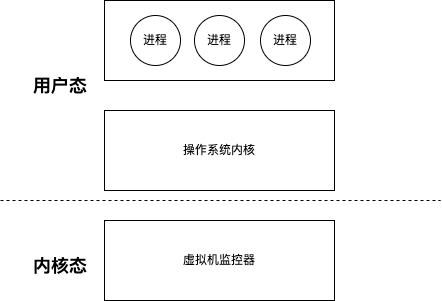
\includegraphics[width=0.75\textwidth]{thesis-images/trap-and-emulate.png}
    \caption{陷入与模拟技术}\label{fig:trap-and-emulate}
\end{figure}

\subsubsection{硬件辅助虚拟化技术} 
硬件辅助虚拟化技术是另一种 CPU 虚拟化技术,用来弥补不可虚拟化架构的缺陷,用来提高虚拟化情况的执行效率。硬件虚拟化对敏感指令的支持主要体现在两个方面。首先,一部分敏感指令不再需要下陷,而是被重定向到虚拟硬件部件,例如 RISC-V 中 vs 开头的寄存器(将在后面的章节中描述);其次,在引入硬件虚拟化技术之后,过去不可虚拟化架构中的敏感指令也都可以通过配置的方式引发下陷,从而被虚拟机监控器处理。\cite{陈海波2019现代操作系统}例如,RISC-V 中引入了一个 hstatus 寄存器,可以用来控制哪些指令需要发生下陷。

\subsection{内存虚拟化技术}

内存虚拟化技术是一种将物理内存资源分配给多个虚拟机或进程使用的技术。它通过软件和硬件的协同控制,在物理内存和虚拟内存之间建立一个中间层,将物理内存分割成多个较小的部分,并将它们分配给不同的虚拟机或进程使用。内存虚拟化技术可以最大化物理内存的利用率,增加系统的灵活性和可靠性,提高虚拟机或进程的性能。常见的内存虚拟化技术包括虚拟内存、内存隔离、内存压缩、内存共享等。  \cite{陈海波2019现代操作系统}
  
为了更加清晰地解释内存虚拟化的作用,本节首先从没有使用系统虚拟化的场景说起。使用系统虚拟化之前,操作系统内核直接运行在最高特权级,因此它有权限管理整个物理地址空间,
“看到的”是从零地址开始连续增长的物理地址空间。使用系统虚拟化后,一台物理主机上可同时运行多个虚拟机。此时每个客户操作系统看到的物理地址也应该从零开始增长。
此外,虚拟机监控器还不允许客户操作系统访问不属于它的物理内存区域。如果此时某个客户操作系统可以访问任意物理内存区域,它就能读取甚至修改其他虚拟机以及虚拟机监控器
的内存中的数据,这破坏了虚拟机的内存隔离,会严重威胁整个系统的安全。  \cite{陈海波2019现代操作系统}
  
因此,内存虚拟化需要满足两个要求:
\begin{itemize}
    \item 第一,为每台虚拟机提供从零开始增长的物理地址空间。
    \item 第二,实现虚拟机之间的内存隔离,每台虚拟机只能访问分配给它的物理内存区域。
\end{itemize}

为了满足这两个要求,这里首先介绍一种新的内存地址:\textbf{客户物理地址},这是虚拟机主机内使用的物理地址,不是真实的、在总线中访存的地址。
真正访存的物理地址被改称为\textbf{主机物理地址}。在虚拟机执行过程中,需要将客户物理地址转换成主机物理地址,然后通过后者访问存储在内存
中的数据和代码。相应地,虚拟机监控器需要提供一种新的地址翻译机制,将客户物理地址翻译成主机物理地址。如图~\ref{fig:mm-virtualization}~ 所示,到目前为止共有三种不同类型的地址:

\begin{itemize}
    \item 第一种是进程和客户操作系统使用的\textbf{客户虚拟地址(Guest Virtual Address, GVA)}。\cite{陈海波2019现代操作系统}
    \item 第二种是客户操作管理的\textbf{客户物理地址(Guest Physical Address, GPA)}。\cite{陈海波2019现代操作系统}
    \item 第三种是 CPU 发送至总线进行访存的\textbf{主机物理地址(Host Physical Address),HPA}。\cite{陈海波2019现代操作系统}
\end{itemize}

引入客户物理地址之后,内存虚拟化技术可拥有以下四个优点:

\begin{itemize}
    \item 第一,可以为每个虚拟机提供一个从零地址开始连续增长的客户物理地址空间,客户操作系统“以为”自己仍然在管理着物理地址空间。\cite{陈海波2019现代操作系统}
    \item 第二,第二阶段地址翻译可提高主机物理内存的使用率;例如,虚拟机监控器将不连续的主机物理地址映射成连续的客户物理地址,从而减少内存碎片。\cite{陈海波2019现代操作系统}
    \item 第三,即使多个虚拟机请求的客户物理内存的大小超出主机物理内存的大小,也可以通过内存虚拟化机制同时支持多台虚拟机的执行。\cite{陈海波2019现代操作系统}
    \item 第四,通过内存虚拟化技术可实现虚拟机之间客户物理地址空间的安全隔离型;因为虚拟机监控器借助第二阶段地址翻译过程限制了每一台虚拟机的地址范围,任何虚拟机不能读写其他吃虚拟机中的物理内存区域。\cite{陈海波2019现代操作系统}
\end{itemize}

接下来将介绍本课题所使用的内存虚拟化的技术。

\begin{figure}[]
    \centering
    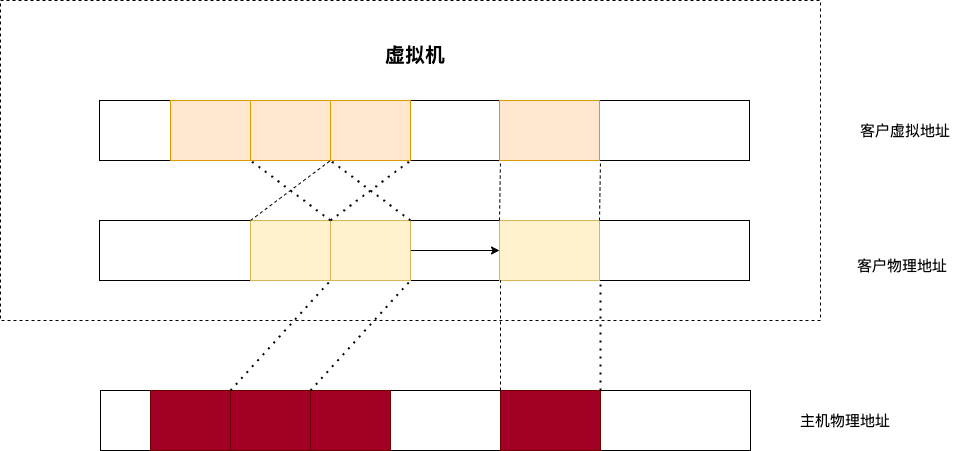
\includegraphics[width=1\textwidth]{thesis-images/mm-virtualization.png}
    \caption{内存虚拟化}\label{fig:mm-virtualization}
\end{figure}



\subsubsection{影子页表机制}
影子页表是一种内存虚拟化技术。在没有影子页表的情况下,客户虚拟地址需要经过两阶段的地址翻译,才可以转换成主机物理地址(首先由客户虚拟地址转换为客户物理地址,再由客户物理地址转换为主机物理地址)。在硬件虚拟化技术出现之前,MMU 只有一个页表,但 MMU 已经被虚拟监控器所使用,那么如何在只有一个页表的情况下同时实现两种地址翻译呢?

在这里就需要引入影子页表(Shadow Page Table, SPT)机制,影子页表是相对于虚拟机内使用的页表而言的概念。虚拟机的操作系统只能为进程配置页表,它会安装页表到 MMU 中,“影子”的含义体现在两个方面。首先,影子页表是虚拟监控器秘密为虚拟机配置的页表,此页表不为虚拟机所见,对其完全透明,更不能被虚拟机更改。其次,影子页表的内容与客户虚拟机的页表高度相关,它的映射内容随着页表内容的改变而改变,就像“影子”一样。\cite{陈海波2019现代操作系统}

图~\ref{fig:spt}~展示了影子页表的构建过程。首先,操作系统在页表中配置客户虚拟地址到客户物理地址的映射,由于虚拟机只能使用客户物理地址,因此他将此页表的客户物理地址写入根页表寄存中。第二步,系统寄存器写入操作引发下陷,陷入到虚拟机监控器中。第三步,虚拟机监控器将遍历客户操作系统安装的页表,并根据表中内容创建一个影子页表。影子页表包含了客户虚拟地址到主机物理地址的映射关系。第四步,虚拟机监控器通过配置影子页表并将页表对应的内存地址设置为只读。第五步,将影子页表跟地址写入根页表寄存器。\cite{陈海波2019现代操作系统}

\begin{figure}[]
    \centering
    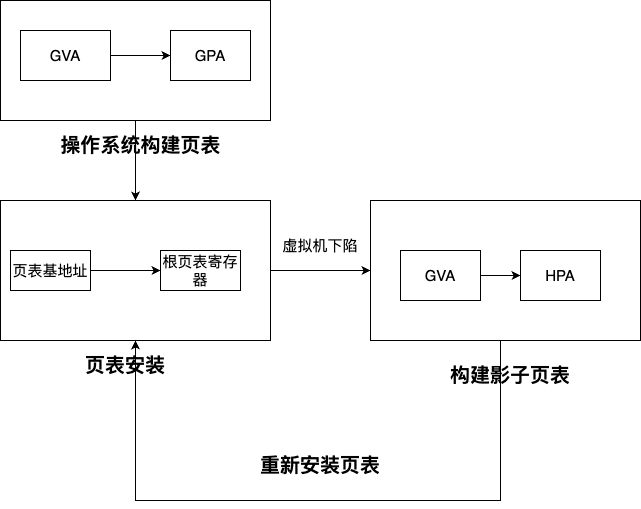
\includegraphics[width=0.75\textwidth]{thesis-images/spt.png}
    \caption{影子页表构建过程}\label{fig:spt}
\end{figure}

\subsubsection{两阶段页表翻译}
两阶段页表翻译是另一种内存虚拟化机制。在一般的硬件辅助虚拟化技术中,硬件会增加虚拟化特权级,并在新增的虚拟化特权级中添加第二阶段页表。此页表记录了客户物理地址到主机物理地址的映射关系。原先虚拟机中使用的页表被称为第一阶段页表,它记录着客户虚拟地址到客户物理地址的映射关系。

\begin{figure}[]
    \centering
    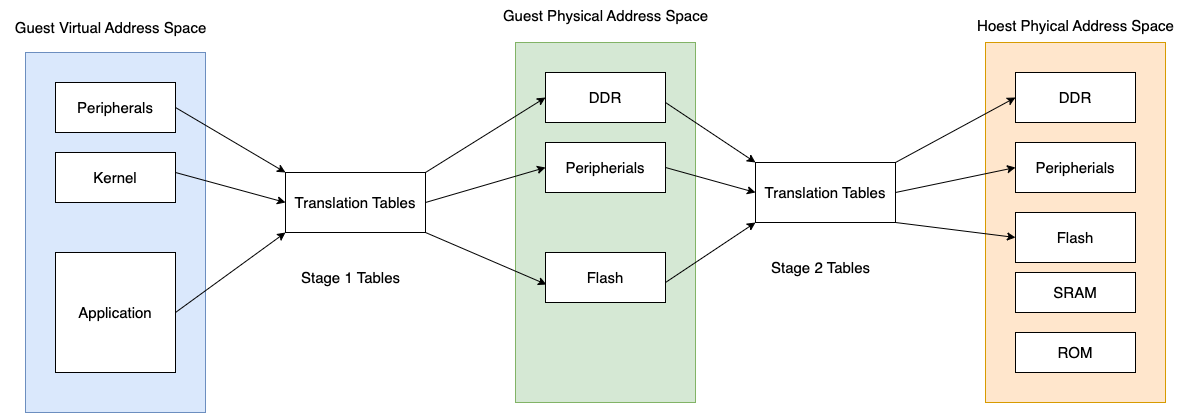
\includegraphics[width=1\textwidth]{thesis-images/two-stage-translation.png}
    \caption{两阶段页表翻译过程}\label{fig:two-stage-translation}
\end{figure}

图~\ref{fig:two-stage-translation}~展示了虚拟化情况下内存访问的机制,在开启了硬件虚拟化的情况下,内存访问会分为两个阶段:客户操作系统控制第一阶段的转换,将客户虚拟地址转换为客户物理地址;虚拟机监控器控制第二阶段的转换,将客户物理地址转换为主机物理地址。\cite{陈海波2019现代操作系统}

\subsection{I/O 虚拟化技术}
操作系统的重要职责之一是管理设备。即使运行在虚拟机之内,客户操作系统也依然“认为”自己需要并有能力管理设备。
然而,出于安全和资源利用率的考虑,虚拟机监控器通常并不允许虚拟机直接管理真实的物理设备,而是利用 I/O 虚拟化技术为
虚拟机提供“假”的设备,例如虚拟磁盘和虚拟网卡;然后虚拟机可以像操作真的设备那样去操作这些虚拟设备。\cite{陈海波2019现代操作系统}

I/O 虚拟化有三个重要功能。首先,它会限制虚拟机对真实物理设备的直接访问。因为物理设备通常需要被多个虚拟机共享,如果
某个虚拟机能够接触物理设备中的数据,将严重威胁其他虚拟机甚至宿主机的安全。其次,I/O 虚拟化会为每个虚拟机提供虚拟设备
接口。以磁盘设备为例,磁盘的起始扇区位置通常存储着重要信息,例如\textbf{主引导记录(Master Boot Record),MBR} 或 
\textbf{全局唯一标识分区表(GUID Partition Table,GPT)}。I/O 虚拟化为虚拟机提供虚拟设备的接口,例如将虚拟机对虚拟
的 1 号磁盘的访问请求翻译成对物理磁盘设备对应山区的请求,从而读取 MBR 数据。再次,I/O 虚拟化可以提高物理设备的资源利用率。
以网卡设备为例,一个虚拟机也许不能占满物理网卡的网络带宽,但如果有多个虚拟机同时使用网卡,就可以有效地提高网卡的带宽利用率。\cite{陈海波2019现代操作系统}

下面介绍本课题所使用到的一些 I/O 虚拟化技术。

\subsubsection{软件模拟方法}

软件模拟的 I/O 虚拟化需要借助模拟或硬件虚拟化的方法捕捉原生驱动(即设备配置的未经修改的驱动程序)的硬件指令,之后在虚拟机监控器
内模拟虚拟设备的行为,并为虚拟机提供 I/O 服务。软件模拟的 I/O 虚拟化通常用作机器指令层,它不要求对驱动程序做任何修改,客户操作系统 
可使用原生驱动程序与设备进行交互。因此软件模拟的 I/O 虚拟化方法也属于全虚拟化技术范畴。\cite{陈海波2019现代操作系统} 

这里以磁盘设备举例,对于磁盘设备来说,一种常见的软件模拟方案是:虚拟机监控器利用文件作为虚拟机的虚拟磁盘,并将虚拟磁盘的扇区位置
映射为文件内的偏移量。因此,读入或写入虚拟磁盘的某个扇区会被翻译成对文件相关偏移位置的数据访问。\cite{陈海波2019现代操作系统}

\subsubsection{设备直通}
设备直通是一种 I/O 虚拟化方法。设备直通意味着让物理设备从虚拟机监控器的管理中脱离,并将其直接交与虚拟机中的原生驱动程序进行管理。这种虚拟化方法的优势显而易见:虚拟机在使用设备时不需要任何虚拟监控器的参与,所以与软件模拟或半虚拟化的方法相比,该方法大大地提高了 I/O 虚拟化的性能。

在使用软件模拟或者半虚拟化进行 I/O 虚拟化的过程中需要首先将数据拷贝到虚拟机监控器中,之后才会被拷贝到设备或者虚拟机中。拷贝数据之前,虚拟机监控器需要将客户物理地址翻译成主机物理地址,并检查地址的合法性。然而,当虚拟机和物理设备直接交互时时,由于缺少虚拟机监控器的中间翻译,驱动程序在发起 DMA 操作时使用的地址只能是物理设备能够理解的主机物理地址(否则将无法完成 DMA 操作)。\cite{陈海波2019现代操作系统}

因此体系结构领域提出了 IOMMU(Input-Output Memory Management Unit)来解决这个问题。与 MMU 类似,IOMMU 也提供了第二阶段地址翻译机制,将设备使用的客户物理地址翻译成主机物理地址,并在翻译过程中进行权限检查。为了阻止直通物理设备对任意主机物理地址的非法访问,虚拟机监控器首先需要为此设备配置 IOMMU 第二阶段页表,以在页表中维护客户地址到主机物理地址的映射关系。在设备进行 DMA 操作时,DMA 所有客户物理地址都会被 IOMMU 页表翻译成主机物理地址,以进行访存操作。如果恶意的虚拟机试图通过 DMA 访问不属于它的内存区域,IOMMU 在翻译时将检查出缺页或权限不足等错误,并通知虚拟机监控器,交由它处理。\cite{陈海波2019现代操作系统}

\subsection{中断虚拟化技术}
中断是操作系统与设备交互时必不可少的机制。当完成某任务后,设备可通过中断异步通知 CPU,以便其进行后续操作。在非虚拟化场景下,来自设备的中断直接唤醒操作系统配置的中断处理函数。在虚拟化场景下,中断可以分为两种类型,一种是物理中断,一种是虚拟中断。物理中断由物理设备直接产生,交给虚拟机监控器。虚拟机监控器一般不允许设备直接将物理中断发给虚拟机。这主要是因为物理设备的中断不一定和某个虚拟机直接相关。\cite{陈海波2019现代操作系统}

在硬件虚拟化技术出现之间,中断虚拟化需要通过软件模拟的方式实现。因此每次产生中断后都会首先陷入到虚拟机监控器,随后虚拟机监控器将根据中断号找到对应的发生中断的虚拟机并进行中断注入。软件模拟的方法实现中断虚拟化会带来较多的虚拟机下陷,因而性能较差。\cite{陈海波2019现代操作系统}

在硬件虚拟化出现了之后,虚拟机监控器可以为虚拟机配置硬件实现的虚拟寄存器,虚拟机可使用这些寄存器控制中断的行为。虚拟机在访问这些寄存器时不会产生任何虚拟机下陷。此外,插入中断的方式也得到了优化。虚拟机监控器可以使用硬件提供的接口插入中断。此中断将在 CPU 恢复虚拟机运行时由硬件自动插入并直接调用对应的中断处理函数。\cite{陈海波2019现代操作系统}

\subsection{RISC-V 指令集}

\subsubsection{RISC-V 指令集概述}
RISC-V指令集是一种开源、自由的指令集架构,旨在提供高效而灵活的处理器设计。RISC-V指令集是一个基于Load-Store架构的指令集,其设计哲学是尽可能简化指令集,使其易于实现。这使得它能够适用于各种不同应用场景,包括嵌入式、移动、桌面和服务器等。

RISC-V指令集的设计是由加州大学伯克利分校的研究人员、工业界专业人士和学术界代表共同完成的。其设计理念源于之前的指令集设计,如ARM和MIPS等。但与其他指令集的设计不同,RISC-V指令集的设计非常注重可扩展性与简洁性。此外,由于RISC-V是一个开源项目,任何人都可以对其进行修改和改进,这使得这个指令集架构适合在开放、共享的环境中快速发展。

\begin{itemize}
    \item 简单易用:RISC-V指令集设计简单,容易学习和理解,并且它的设计思想与CISC指令集不同,因此在使用RISC-V指令集开发应用程序时,可编写更简单、更清晰的代码。
    \item 可扩展:在RISC-V中添加额外的指令是非常容易的,这可以为某些需求定制应用程序提供最大灵活性。比如,RISC-V可以添加自定义指令,以优化特定的应用程序。
    \item 高分辨率的架构:RISC-V指令集的设计使得实现高分辨率的机器架构变得容易。此外,高分辨率的架构具有更好的指令选择和解码效率,因此可以在更少的周期内完成更多的操作。
    \item 开源:RISC-V指令集是一项开源技术,其设计体现了大量的开放和共享原则。这种开源的特性使得RISC-V指令集得以在全球范围内获得广泛的认可和使用,为整个计算机行业产生巨大的影响力。
\end{itemize}

RISC-V 从诞生至今一直在高速发展,短短几年时间的出货量已经达到了 100 亿颗。对于中国来说,其他的主流 CPU 架构如 x86 和 ARM 具有很强的垄断性,世界市场上主流 CPU 都被 x86 和 ARM 垄断,
而它们都是美国公司的产权。因此为了突破在芯片上卡脖子的问题,RISC-V 在目前来说是一个极好的选择。

\subsubsection{RISC-V 特权级架构}
RISC-V特权级别分为 4 种,从层级逐渐递增,包括机器模式(Machine Mode)、特权模式(Supervisor Mode)、和用户模式(User Mode),在最新一版的标准中 RISC-V 加入了虚拟化扩展功能(Hypervisor Extension),关于 RISC-V 虚拟化扩展将在之后的章节进行具体讲解。

机器模式是运行裸机程序的模式,这时处理器处于最高特权级别,可以访问所有资源。机器模式包括了所有的核心机器操作,如虚拟内存管理、异常处理、中断控制等。
特权模式是处理器为执行特权级别软件而进入的最高特权级别,用于执行操作系统和底层驱动程序等特权级别软件。特权级别软件可访问对应的特权寄存器和指令集,以完成和控制对其特权等级和基础硬件资源的访问。

用户模式则是普通应用程序所运行的模式,它只能访问受限的地址空间和指令集,以保护操作系统和硬件免受非法操作的损害。

而虚拟化模式(将在下一节介绍)是为了 RISC-V 虚拟化而设置的,它可以在硬件层面为操作系统提供虚拟化加速的能力。

\begin{figure}[]
    \centering
    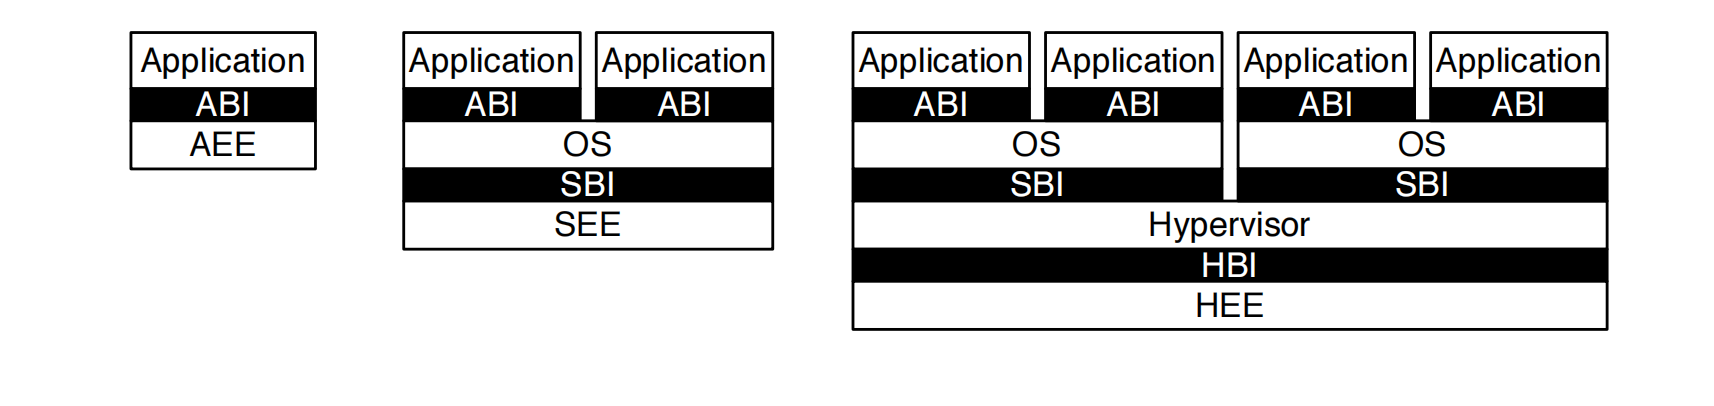
\includegraphics[width=1\textwidth]{thesis-images/riscv-privilege.png}
    \caption{RISC-V 特权级\cite{riscv_isa}}\label{fig:riscv-privilege}
\end{figure}

图~\ref{fig:riscv-privilege}~展示了 RISC-V 不同特权级的情况。需要注意的是,RISC-V 特权级并非要同时存在,对于简单的嵌入式设备, 
只需要支持 M mode 和 U mode 即可,U mode 通过 ABI 调用获取 \textbf{应用执行环境(application execution environment, AEE)} 的服务。
通用操作系统需要支持 M mode、S mode 和 U mode,其中 S mode 通过 SBI 调用获取 \textbf{监管执行环境(supervisor execution environment, SEE)} 的服务。
虚拟机监控器则需要运行在同时支持 M mode,S mode 和 H extension 和 U mode 的处理器上,虚拟机监控器通过 HBI 调用 \textbf{虚拟机执行环境(hypervisor exection environment, HEE)} 并向上提供监管执行环境。\cite{riscv_isa}

\subsubsection{RISC-V 虚拟化扩展}
为了支持 RISC-V 虚拟化,RISC-V 委员会提出了 RISC-V 虚拟化扩展并在 2021 年 11 月被正式通过并发布了 1.0 版本。RISC-V 虚拟化扩展功能将原有的 RISC-V Supervisor mode 修改为了 hypervisor-extended supervisor mode(HS-mode),可以在其中运行 hypervisor 或者可以运行客户操作系统的主机操作系统。RISC-V 虚拟化扩展也提供了从客户物理地址到主机物理地址的翻译,以此来为客户操作系统实现虚拟内存和虚拟 MMIO。通用的运行在 S mode 上的操作系统可以不加修改地运行在 HS-mode 或者 VS-mode。\cite{riscv_isa}

当运行在 HS-mode 下,hypervisor 或者主机操作系统通过 SBI 和真实物理机器进行交互(就像运行在 S-mode 的操作系统一样),同时,运行在 HS-mode 的 hypervisor 或者主机操作系统也应当实现 SBI 调用以向上层操作系统提供服务。\cite{riscv_isa}


% \begin{figure}[]
%     \centering
%     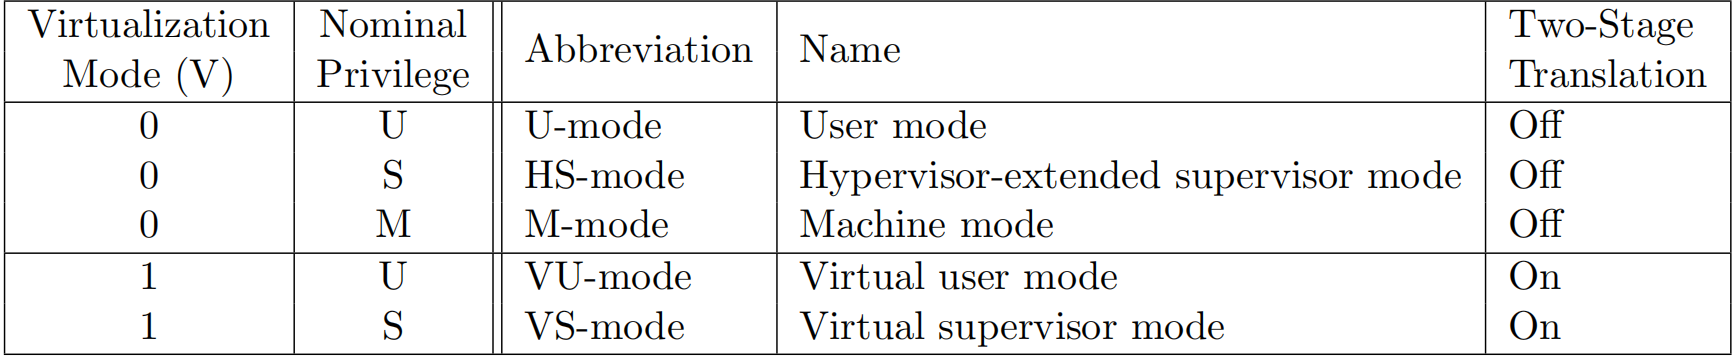
\includegraphics[width=1\textwidth]{thesis-images/h-priv.png}
%     \caption{RISC-V 虚拟化扩展}\label{fig:h-priv}
% \end{figure}

\begin{table}[htbp]
    \caption{RISC-V 虚拟化扩展}\label{tab:h-priv}
    \vspace{0.5em}\centering\wuhao
    \begin{tabular}{*{3}{p{2cm}}*{2}{p{4cm}}}
    \toprule[1.5pt]
    Virtualization Mode(V) & Nomainal Privilege & Abbreviation & Name & Two-Stage Translation \\
    \midrule[1pt]
    0 & U & U-mode & User mode & Off \\
    0 & S & HS-mode & Hypervisor-extened supervisor mode & Off \\
    0 & M & M-mode & Machine mode & Off \\
    1 & U & VU-mode & Virtual user mode & On \\
    1 & S & VS-mode & Virtual supervisor mode & On \\
    \bottomrule[1.5pt]
    \end{tabular}
    \vspace{\baselineskip}
    \end{table}

当开启了 RISC-V 虚拟化扩展后,RISC-V 特权级模式和传统的特权级略有不同。表~\ref{tab:h-priv}~展示了添加了虚拟化扩展后的 RISC-V 特权级列表。新增的 V 模式表示当前程序是否运行在虚拟化模式下,当 V=1 时,当前 hart 可能运行在虚拟监管模式(VS-mode)或者虚拟用户模式(VU-mode),当 V=0 时,当前 hart 可以运行在 M-mode,HS-mode 或在 HS-mode 运行的操作系统下的 U-mode。是否开启虚拟化模式也决定当前是否开启两阶段页表翻译,上表展示了当前 hart 所有可能的特权级状态。\cite{riscv_isa}

RISC-V 为了支持虚拟化功能,除了使用原有的 S-mode 寄存器外,还在 HS-mode 添加了一些寄存器,这些寄存器可以用于提供两阶段页表翻译和对于运行在 VS-mode 的客户操作系统的行为进行控制,添加的 HS-mode 寄存器有:hstatus, hedeleg, hideleg, hvip, hip, hie, hgeip, hgeie, henvcfg, henvcfgh, hcounteren, htimedelta, htimedeltah, htval, htinst, 和 hgatp。\cite{riscv_isa}下面将对在 HS-mode 添加的某些重要的寄存器的功能做一个简要说明:

\begin{itemize}
    \item hstatus: hstatus 提供类似于 mstatus 的功能,用于跟踪和控制 VS-mode 下客户操作系统的异常行为。\cite{riscv_isa}
    \item hedeleg 和 hideleg: 用于设置是否将中断和异常代理到运行在 VS-mode 的客户操作系统上。\cite{riscv_isa}
    \item hvip, hip, hie: hvip 是一个可读写寄存器,可以用于向 VS-mode 注入虚拟终端,而 hip,hie 则和 sip,sie 提供相同的能力。\cite{riscv_isa}
    \item hgeip, hgeie: hgeip 是一个只读寄存器,用来表示当前 hart 正在等待的 guest 外部中断;hgeie 是一个可读写寄存器,提供了对于当前 hart guest 外部中断的使能。\cite{riscv_isa}
    \item hcountern: 用于控制 VS-mode 下时钟使能,理论上必须实现。\cite{riscv_isa}
    \item htval: 当发生异常且陷入 HS-mode 时,关于地址错误信息将被写入到 htval 寄存器中。 \cite{riscv_isa}
    \item htinst: 当发生异常且陷入 HS-mode,关于异常指令将被写入到 htinst 寄存器中。\cite{riscv_isa}
    \item hgatp:用于第二阶段页表翻译,硬件将根据写入 hgatp 的页表信息找到跟页表地址并进行页表翻译。\cite{riscv_isa}

\end{itemize}

\section{小结}

本章首先对于当前工业界与学术界相关的工作做了简要介绍,之后介绍了在本次课题中所使用到的相关的技术,
包括虚拟化技术,并对 CPU 虚拟化、内存虚拟化、I/O 虚拟化、中断虚拟化等理论做了说明。同时也对 RISC-V 指令集架构
做了简短的介绍。

\chapter{系统的设计与实现}

本课题实现了两版基于 RISC-V 平台的虚拟化软件,第一版为 hypocaust,不依赖于任何硬件虚拟化特性,完全使用软件的特权级陷入与模拟进行实现,最终可以启动一个小型的带文件系统的操作系统;第二版为 hypocaust-2,使用了 RISC-V Hypervisor Extension 硬件辅助虚拟化进行实现,最终可以运行 rCore-Tutorial-v3, RT-Thread, Linux mainline 等操作系统,两版操作系统全部使用 Rust 语言进行实现,下面将详细讲述两版 hypervisor 的设计与具体实现。

\section{hypocaust 总体设计}
hypocaust 是一个使用 Rust 语言编写的软件全虚拟化 Type-1 hypervisor,使用了 S-mode 下陷与模拟技术。

\begin{figure}[]
    \centering
    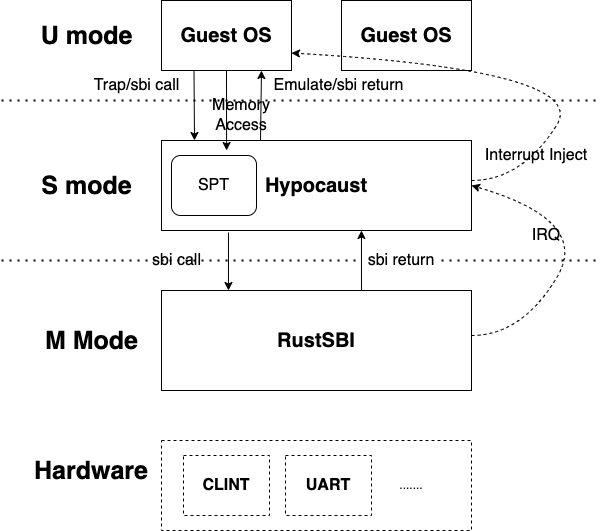
\includegraphics[width=0.75\textwidth]{thesis-images/hypocaust-architecture.png}
    \caption{hypocaust 整体架构}\label{fig:hypocaust-arch}
\end{figure}

图~\ref{fig:hypocaust-arch}~展示了 hypocaust 的设计架构,hypocaust 运行在 M mode 的 RustSBI 上,RustSBI 可以通过处理 sbi call 来为 hypocaust 提供服务,例如,hypocaust 可以通过 sbi call 来进行输入输出与设置时钟中断。同时,hypocauat 也为运行在 U mode 的 guest os 提供服务,hypocaust 需要为 guest os 提供 sbi 服务并在 guest 执行特权级指令时模拟并返回。  

当 hypocaust 进行内存的访问时,客户操作系统将不会遍历由客户自己维护的页表,而是遍历由虚拟机监控器维护的影子页表,便于直接将客户虚拟地址转换成主机物理地址。每当客户操作系统切换页表时总会陷入虚拟机监控器,虚拟机监控器通过遍历客户页表并对其进行重新映射从而构造出影子页表。

hypocaust 的中断虚拟化是通过中断注入来实现的,当 hypocaust 收到由 SBI 发送的中断请求时,hypocaust 会获取到对应的中断请求 ID,随后 hypocaust 会讲对应的中断请求 ID 注入到对应的 CPU 核中(这主要是通过 PLIC 获取中断请求号的地址来识别)。

hypocaust 的 IO 虚拟化通过设备透传来实现,即暴露对应的 MMIO 地址给客户操作系统,客户操作系统从而可以直接控制设备,不需要经过虚拟机监控器的干预,具有最高的 IO 性能。
 


\section{hypocaust-2 总体设计}
hypocaust-2 是 hypocaust 项目的继任者。hypocaust-2 使用了 RISC-V 提供的硬件辅助虚拟化技术,即 Hypervisor Extension 来进行设计与实现,相比于完全使用软件来实现的虚拟机监控器,hypocaust-2 拥有更高的性能,并且基于软硬件协同的设计,使得代码结构更为精简,维护起来更为简单;但是缺点是 hypocaust-2 只能运行在实现了虚拟化扩展的硬件上执行,而 hypocaust 可以在任何 RISC-V 芯片上执行。

\begin{figure}[]
    \centering
    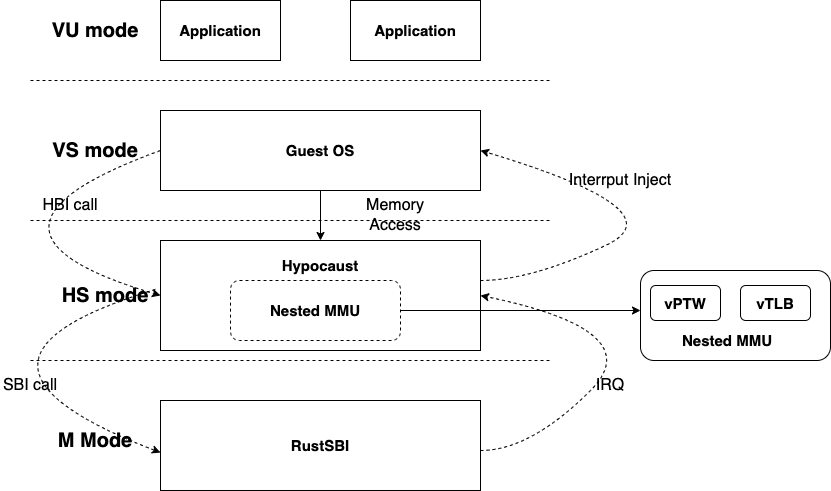
\includegraphics[width=1\textwidth]{thesis-images/hypocaust-2-arch.png}
    \caption{hypocaust-2 整体架构}\label{fig:hypocaust-2-arch}
\end{figure}

图~\ref{fig:hypocaust-2-arch}~展示了 hypocaust-2 的总体架构,在开启了 RISC-V 虚拟化扩展的情况下,hypocaust-2 运行在 HS-mode,接受由运行在 M-mode 的 RustSBI 提供的服务,并向运行在 VS-mode 的客户操作系统提供服务。

当客户操作系统发起内存访问时,不同于 hypocaust 使用影子页表,hypocaust-2 依赖于硬件虚拟化提供的两阶段页表翻译机制,在硬件上需要维护一个 Nested MMU,其中包括 vPTW 与 vTLB 用于维护两阶段页表翻译的页表遍历与快表查找,由于本课题的重点
不是关于微体系结构的设计与实现,因此对于不对于硬件的设计进行详细说明。

hypocaust-2 的中断虚拟化与 IO 虚拟化的实现与 hypocaust 基本相同,这里不再赘述。

\section{CPU 虚拟化}
关于 CPU 虚拟化的原理在之前的章节中已经做了介绍,本节不再做赘述,本节将具体介绍 hypocaust 与 hypocaust-2 CPU 虚拟化的设计与实现。因此,在设计 CPU 虚拟化的过程中,首先有几个问题值得我们考虑:
\begin{enumerate}
    \item 对于每个 hart 的 vCPU 需要维护哪些状态与寄存器?
    \item hypervisor 如何处理读写 CSR 指令和其他特权指令?
    \item hypervisor 是如何为 guest 提供 sbi 服务的?
    \item hypervisor 如何在处理之后返回 guest 继续执行?
\end{enumerate}


\subsection{CPU 虚拟化在 hypocaust 中的设计与实现}
由于 hypocaust 是使用纯软件实现的虚拟机监控器,因此对于 CPU 虚拟化采用的是陷入与模拟技术。为了实现陷入与模拟技术,除了需要保存一些虚拟机监控器与客户操作系统上下文切换所必需的信息,还需要保存一些特定的信息用于进行模拟,在 hypocaust 中将这个信息取名叫做shadow\_state。这里我们由里及外,一层一层地分析 hypocaust 为 CPU 虚拟化所维护的状态。shadow\_state 所保存的信息如下表所示:


\begin{table}[htbp]
\caption{shadow\_state 结构体}\label{tab:table1}
\vspace{0.5em}\centering\wuhao
\begin{tabular}{p{5cm}p{5cm}p{5cm}}
\toprule[1.5pt]
成员变量 & 内容 & 描述\\
\midrule[1pt]
csrs & sstatus, sie, sip, stvec, sscratch, sepc, scause, stal, satp, mtimecmp & 控制状态寄存器\\
shadow\_page\_tables & ShadowPageTable<P> & 影子页表列表\\
interrupt &  - & 是否发生中断 \\
conseutive\_satp\_switch\_count & - & 连续切换根页表寄存器的次数 \\
\bottomrule[1.5pt]
\end{tabular}
\vspace{\baselineskip}
\end{table}

表~\ref{tab:table1}~展示了 hypocaust 所维护的 shadow\_state 的结构,由于 hypocaust 的运行客户操作系统的基准是 rCore-Tutorial-v3,在调研了 rCore-Tutorual-v3 使用了哪些控制状态寄存器后,列出了需要模拟的控制状态寄存器,除了控制状态寄存器外,shaodw\_state 还需要维护影子页表、是否发生中断以及连续切换根页表寄存器的次数,这些状态的作用将在之后的章节进行介绍。

\begin{table}[htbp]
    \caption{hypocaust 为客户操作系统所维护的状态}\label{tab:table2}
    \vspace{0.5em}\centering\wuhao
    \begin{tabular}{p{7.5cm}p{7.5cm}}
    \toprule[1.5pt]
    成员变量 & 描述\\
    \midrule[1pt]
    trap\_cx\_ppn & 上下文切换物理页\\
    trap\_cx & 上下文切换保存的状态\\
    shadow\_state&维护的影子状态\\
    guest\_id&客户操作系统标识号\\
    smode&记录当前 guest 是运行在 S-mode 还是 U-mode\\
    virt\_device&维护的虚拟设备\\
    \bottomrule[1.5pt]
    \end{tabular}
    \vspace{\baselineskip}
    \end{table}


表~\ref{tab:table2}~展示了 hypocaust 所有为客户操作系统维护的状态,除了之前提到的 shadow\_state,还包括 trap\_cx\_ppn,用于记录上下文切换时分配的物理页号;trap\_cx 用于 hypervisor 与 guest 进行上下文切换时保存的状态,其中包括 32 个通用寄存器,一些 S-mode 控制状态寄存器,hypervisor 栈指针,hypervisor 页表地址以及 trap\_handler 地址;guest\_id,用于标识客户操作系统的 id;smode,表示当前客户操作系统认为自己运行在哪个特权级(虚拟化出来的特权级,实际上全都运行在用户态)以及 virt\_device,用于表示虚拟化出来的设备。

\begin{figure}[]
    \centering
    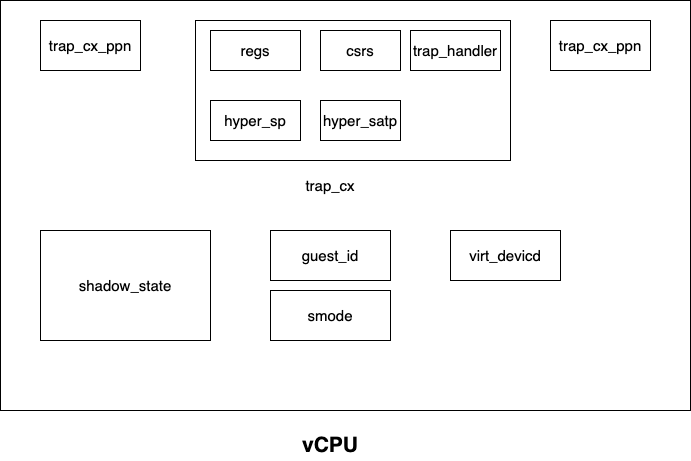
\includegraphics[width=1\textwidth]{thesis-images/hypocaust-vcpu.png}
    \caption{hypocaust vCPU}\label{fig:hypocaust-vcpu}
\end{figure}

为了使读者对于 vcpu 的构造有一个直观的认识,图~\ref{fig:hypocaust-vcpu}~展示了 hypocaust 的 vCPU的整体架构,在 Rust 编程语言中使用 struct 进行实现。


在之前的部分中介绍了 hypocaust 需要存储哪些信息以维护 vCPU 的状态,现在将介绍当 guest 执行到特权级指令并陷入 S mode 的过程中,hypocaust 是如何进行处理的。

\begin{figure}[]
    \centering
    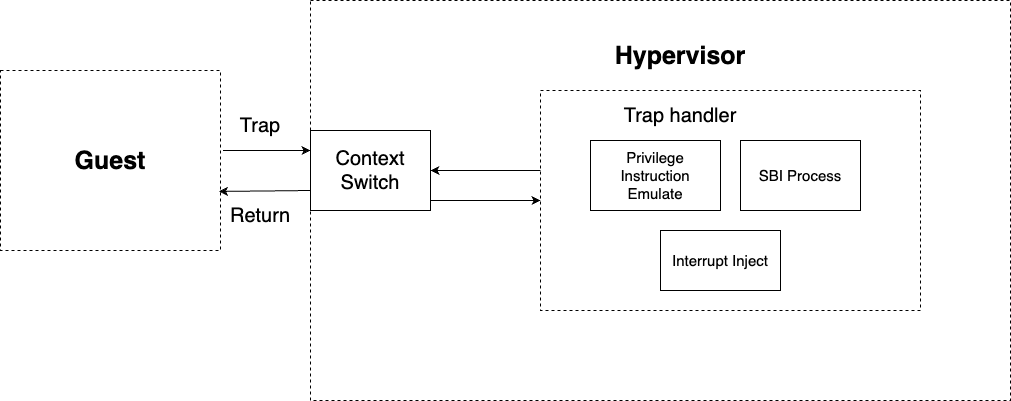
\includegraphics[width=1\textwidth]{thesis-images/hypocaust-trap.png}
    \caption{hypocaust 陷入处理流程}\label{fig:hypocaust-trap}
\end{figure}

图~\ref{fig:hypocaust-trap}~展示了 guest 陷入 hypervisor 后处理的一般性场景,首先当硬件检测到 guest 执行了特权指令或者发生了中断后,由 guest 所在的 U mode 陷入到 S mode 中,首先将 pc 切换到由 stvec 寄存器指向的中断向量地址,这段指令将会执行一段上下文切换代码,将需要保存的 guest 寄存器保存到一段 Trap Context 地址中(由 hypervisor 进行分配与维护,将在内存虚拟化章节中进行详细讲解),随后跳转到陷阱处理子系统(由 trap\_handler 维护),陷阱处理子系统包含三个部分,分别是特权指令处理,SBI 调用处理以及中断注入处理(将在下节进行描述)。在执行了陷阱处理子系统后,将会再次执行上下文切换并返回到 guest 中继续执行。

\begin{figure}[]
    \centering
    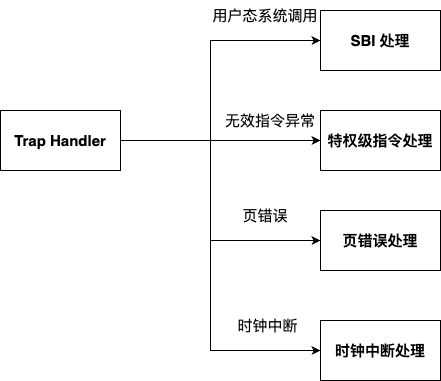
\includegraphics[width=0.65\textwidth]{thesis-images/trap-handler.png}
    \caption{Trap Handler 处理流程}\label{fig:trap-handler}
\end{figure}

接下来将详细描述关于特权级指令处理以及 SBI 调用处理的实现。图~\ref{fig:trap-handler}~展示了 trap\_handler 的具体流程中,在 trap\_handler 的实现中,使用 riscv crate 可以根据 scause 的值来对异常原因进行分类,当发生无效指令异常时将会被派发到 inst\_fault 进行处理,当检测到为用户态系统调用时,将被派发到 sbi\_vs\_call 进行处理,关于页错误处理和时钟中断处理将在之后的章节进行详细描述。  
  
inst\_fault 首先会解析发生异常所在地址的指令进行解析,如果特权级指令表示读取某些 CSR,hypervisor 将会将维护的该寄存器的值拿出来并放入 a0 寄存器以返回;同样地,对于写入 CSR 指令,将会将值写入维护的 CSR 状态中,值得注意的是对于某些寄存器的写入还需要伴随附加操作,例如对于 satp 的写入操作可能需要进行影子页表的构建。其他特权级指令类似 sret 则需要按照特权级手册进行模拟,这里不再赘述。 

sbi\_vs\_call 的处理与 inst\_fault 类似,需要首先解析指令,对于不同类型的 sbi call,有些可以直接发送指令到 RustSBI 进行处理,有些则需要进行生动模拟。

\subsection{CPU 虚拟化在 hypocaust-2 中的设计与实现}

hypocaust-2 作为 hypocaust 的继任者,在很大程度上继续延续了 hypocaust 的设计,但是由于 hypocaust-2 使用了 RISC-V Hypervisor Extension 作为硬件虚拟化辅助扩展,因此在设计上也有一些不同与取舍,同时,有了对于 hypocaust 设计的经验,hypocaust-2 对于一些设计更加的简洁与合理,本章主要描述 hypocaust-2 在 CPU 虚拟化方面与 hypocaust 的相同点与不同点。

关于硬件辅助虚拟化的原理已经在第二章介绍过了,
本节不再赘述。
hypocaust-2 与 hypocaust 在 CPU 虚拟化表现的主要区别之处在于:
hypocaust 需要通过在陷入后模拟特权级指令的行为,将控制状态寄存器写入由 shadow\_state 维护的 csr 中。
对于 hypocaust-2 来说,硬件将会为运行在 VS-mode 的客户操作系统维护一套 vs 开头的控制状态寄存器,
当客户操作系统尝试读写 s 开头的控制状态寄存器时,硬件将会自动读取或写入 vs 的寄存器,而不需要对于陷入的特权级指令进行模拟。
同时,对于 sfence.vma 等需要刷新 TLB 的特权指令,开启了硬件虚拟化特性的硬件将会实现 vTLB 部件,用于虚拟化第一阶段页表的刷新。

相比于 hypocaust,hypocaust-2 在为客户操作系统维护的数据结构方面无需维护 shadow\_state 的信息。同时,为了使得设计更加的简洁,移除了关于 trap\_cx 以及 trap\_cx\_ppn 的维护信息,代替的是将分配的 Trap Context 映射到固定的虚拟地址(将在之后的内存虚拟化中详细介绍),从而当 hypocaust-2 需要访问 Trap Context 的时候,只需从固定的虚拟地址中获取信息即可。

对于 Trap Handler 的实现方面与 hypocaust 的实现流程大致相同,唯一不同的是无需再为无效指令异常单独进行处理,这些异常的处理将会被代理到 VS-mode 由客户操作系统进行处理。sbi call 将会被归类到 Virtual Supervisor Environment Call 中;同时,Hypervisor Extension 允许 hypervisor 通过 hstatus 自定义陷入特权指令,这些指令则被归类于 Virtual Instruction 中,因此这些也需要进行单独处理。

\section{内存虚拟化}

\subsection{内存虚拟化在 hypocaust 中的实现}

在之前的章节中介绍了 hypocaust 是如何在没有硬件辅助虚拟化的情况下是如何设计与实现 CPU 虚拟化的,本节中将介绍 hypocaust 的内存虚拟化的设计与实现。回顾上节,我们提到对于写入 satp 寄存器的操作,需要额外进行一些操作,这是由于 guest 写入 satp 寄存器的时候表明进行了页表切换,因此此时需要进行影子页表的建立以便可以建立从 GVA(客户虚拟地址)到 HPA(主机物理地址)的页表映射。

若要为 hypervisor 实现内存虚拟化,至少需要为 hypervisor 实现以下几个功能:
\begin{itemize}
    \item 建立由 GVA 翻译到 HPA 的影子页表。 
    \item 当 Guest 修改页表时需要对客户页表与影子页表进行同步。  
\end{itemize}
  
这样,当客户操作系统访问客户虚拟内存时,MMU 将会经过影子页表的转换成主机物理地址,从而实现了内存虚拟化。下面将详细描述这些功能的设计与实现。  
  
首先在对 hypocaust 中影子页表的具体设计与实现进行介绍时需要先说明一下 hypocaust 的内存布局,只有在明确了内存布局后才可以进一步进行内存虚拟化的设计。

\begin{table}[htbp]
    \caption{hypocaust 内存布局}\label{tab:table3}
    \vspace{0.5em}\centering\wuhao
    \resizebox{\textwidth}{!}{
    \begin{tabular}{cccc}
    \toprule[1.5pt]
    客户虚拟地址&客户物理地址&主机物理地址&内存布局描述\\
    \midrule[1pt]
    0x80000000 - 0x80200000&0x80000000 - 0x80200000&0x80000000 - 0x80200000&RustSBI\\
    0x80200000 - 0x88000000&0x80200000 - 0x88000000&0x80200000 - 0x88000000&Hypocaust\\
    0x88000000 - 0x90000000&0x88000000 - 0x90000000&0x88000000 - 0x90000000&GuestOS 1\\
    0x90000000 - 0x98000000&0x90000000 - 0x98000000&0x90000000 - 0x98000000&GuestOS 2\\
    0x98000000 - 0x100000000&0x98000000 - 0x100000000&0x98000000 - 0x100000000&GuestOS 3\\
    0x100000000 - 0x108000000&0x100000000 - 0x108000000&0x100000000 - 0x108000000&GuestOS 1 SPT\\
    0x108000000 - 0x110000000&0x108000000 - 0x110000000&0x108000000 - 0x110000000&GuestOS 2 SPT\\
    0x100000000 - 0x108000000&0x100000000 - 0x108000000&0x100000000 - 0x108000000&GuestOS 3 SPT\\
    \bottomrule[1.5pt]
    \end{tabular}
    }
    \vspace{\baselineskip}
    \end{table}

表~\ref{tab:table3}~展示了 hypocaust 客户虚拟地址、客户物理地址、主机物理地址的地址映射情况,本项目的地址状况考虑了 3 个客户操作系统的扩展,并且将影子页表的地址依次映射到高地址。这样做的好处在于,影子页表与客户页表的映射是恒等映射,便于调试与维护,然而不足在于这将会浪费较多的地址空间。作为一个实验性的虚拟机监控器项目,在最初的时候使用最简单的方法构建出一个易于维护和调试的成品比在某方面都做优化的复杂成品更为易于掌控。  

在表~\ref{tab:table3}~中仍有一些内存空间没有被提及,例如,客户操作系统与虚拟机监控器进行上下文切换的代码被映射到跳板页中,sv39 的最高地址,即 0xFFFFFFFFFFFFF000。对于每个 hart 的 Trap Context 的虚拟地址从跳板页地址依次向下映射。

在明确了 hypocasut 的内存布局后,接下来将详细介绍关于 hypocasut 对于影子页表的设计与实现。

首先需要明确的一点是,影子页表的构建并不是针对客户操作系统的,而是针对每个进程的,这个问题在实现时也曾经困扰过我很久。
因此,虚拟机监控器需要为每个虚拟机的每个进程都要创建一个影子页表,并且应当可以通过 satp 的值查找到对应的影子页表,因此,
在 Rust 编程语言中可以使用 BTreeMap 来建立一个映射,用于可以通过 satp 快速找到对应的影子页表结构。
除此之外,虚拟机监控器还需要维护当前正在使用的客户 satp 的值以便安装页表以及当客户操作系统在读写 satp 来决定是否需要更新。

构建影子页表的步骤如下:
\begin{enumerate}
    \item 客户操作系统向 satp 寄存器写入值。
    \item 执行特权级指令将会陷入 S-mode 交由虚拟机监控器处理。
    \item 虚拟机监控器拿到写入的 satp 的值,从 BTreeMap 中进行查找,若能找到,说明该页表对应的影子页表已经被创建,在创建的情况只需进行页表安装并返回即可;若没有找到,则说明该页表对应的影子页表仍然没有被创建。
    \item 当写入页表对应的影子页表没有被创建时,需要为页表创建对应的影子页表。在表~\ref{tab:table3}~中提到影子页表对应的地址空间并非是通过内存分配器分配的而是直接映射在高地址空间,因此构建影子页表需要对客户页表全部页表项都进行一次 page walk 并且将最终的叶子页表项的物理地址进行翻译,即将 GPA 翻译成 HPA 并写入影子页表项中。
    \item 在上一步的过程中需要标记哪些页表项对应页表地址,需要单独将这些页表项设置为只读。
    \item 为影子页表映射跳板页以及 Trap Context 页,以便当客户操作系统陷入到跳板页进行执行。
    \item 将对应的 satp 以及对应的影子页表结构加入到维护的 BTreeMap 结构中。
    \item 虚拟机监控器安装影子页表并返回客户操作系统执行。
\end{enumerate}


以上就是 hypocaust 构建影子页表的构建流程。在步骤中我们提到需要为影子页表的页表部分单独设置为只读权限,那么为什么需要这样做呢?试想一种情况,若客户操作系统安装了页表后需要修改已经创建了的内核页表或者修改用户页表,那么在没有将页表设置为只读情况下,虚拟机监控器将无法监控到这些情况,影子页表将会与客户页表不同步,将会造成非常严重的后果。

因此,当影子页表将对应的页表物理地址设置为只读后,当客户操作系统尝试去写页表的时候将会造成内存页异常,随后触发陷阱陷入到虚拟机监控器中,hypocaust 同步客户页表与影子页表的步骤如下所示:
\begin{enumerate}
    \item 客户操作系统修改页表陷入虚拟机监控器。
    \item 虚拟机监控器获取触发异常的地址和值。
    \item 虚拟机监控器根据触发异常的地址分析修改的是非叶子页表项还是叶子页表项,并对影子页表做同步的修改并返回。
\end{enumerate}

以上所分析的算法是理想算法,但是分析修改的是叶子页表项还是非叶子页表项则较为麻烦,一开始是看低十位的标志位来分析,但是编译器优化有时只会修改低八位而无法分析全部的页表项信息,而且有时分析的结果也不正确,对本项目的实现造成了很大的困扰。

因此作为工程项目的取舍,只好在每次修改时再全部走一遍 page walk 并对于不匹配的页表项进行更新,这样会极大地拉低性能,但为了内存映射的正确性也只好如此。

\subsection{内存虚拟化在 hypocaust-2 中的实现}
与 hypocaust 不同,hypocaust-2 使用了硬件辅助虚拟化扩展的两阶段页表技术,因此无需在进行影子页表的构建与安装以及同步客户页表以及影子页表等一系列操作。RISC-V Hypervisor Extension 提供了两个新增的寄存器: 

vsatp 将负责从客户虚拟地址翻译到客户物理地址,也就是第一阶段页表翻译,由客户操作系统负责;hgatp 负责从客户物理地址翻译到主机物理地址,也就是第二阶段页表翻译,由虚拟机监控器负责。

对于第一阶段页表翻译,是由客户操作系统来负责的,因此本课题不需要对其进行实现。hypocaust-2 所要实现的重点是第二阶段页表翻译。根据 RISC-V 特权级标准规定,RISC-V 第二阶段的根页表需要设置为 16KiB 并且地址也需要进行 16KiB 对齐。为了实现对于之前的页表功能的复用,本项目在 Rust 中定义了一个 GuestPageTable trait,并且将页表结构体作为范型实现了这个 trait。因此一个 Sv39 的页表可以写成 PageTableSv39<PageTable> 和 PageTableSv39<GuestPageTable>,分别表示普通的 Sv39 页表以及虚拟化 Sv39 页表。

这里有必要介绍一下关于 Rust 语言的 trait 特性,trait 是一种特殊的 Rust 类型,它定义了一组方法,可以用于实现特定行为或功能的抽象。这些方法被 Rust 的结构体类型实现,从而达到对某个行为或功能的具体化。
trait 机制使得 Rust 类型系统更加灵活和强大,因为它允许在不同的类型之间共享通用的行为或功能,从而减少了代码的重复。  
  
在上述的例子中,GuestPageTable 和 PageTable 除了分配根页表的方法不同,其他方法均是相同的,因此 GuestPageTable 只需在继承 PageTable 的基础上增加一个 alloc\_16\_page() 方法即可,这极大地减少了代码量的重复。

除此之外,一个不容易注意的细节是,RISC-V 虚拟化扩展标准提及需要为客户操作系统的页表项全部映射为用户态。并且,为了便于操作与维护,hypocaust-2 将所有客户操作系统地址全部映射为可读可写可执行与用户模式,这样更简单且易于维护。若不将所有页表项加入可执行的标志,当客户操作系统为应用程序分配内存并且执行时就会造成异常。

因此,在构建了以上的结构后,构建第二阶段页表映射就和普通的页表映射一样简单而无需进行复杂的影子页表构建和客户页表与影子页表的同步了。

\subsection{hypocaust 与 hypocaust-2 中对于 PageFault 的异常处理}
本章节主要讲述关于 hypocaust 与 hypocaust-2 对于 \textbf{PageFault(页异常)} 的处理流程,本章节实际上不能算是
关于虚拟机监控器实现中的主干环节,但我认为这仍然是一个值得讨论的问题。

对于 hypocaust 来说,由于其是一个纯软件实现的虚拟机监控器,因此无法使用硬件虚拟化提供的硬件特性,因此当客户操作系统发生 PageFault 并陷入 
虚拟机监控器时,hypocaust 可以直接获取到客户操作系统的异常指令地址与发生异常的地址,且这两个地址均为主机物理地址。因此 hypocaust 可以直接
对于获得发生异常的指令与地址进行处理。

对于 hypocaust-2 来说情况则发生了变化,由于 hypocaust-2 启用了两阶段页表翻译,因此在 \textbf{stval} 与 \textbf{sepc} 中获得的地址并非真实的
主机物理地址,而是客户虚拟地址,因此不可以直接对这两个寄存器进行使用。幸运的是,RISC-V 虚拟化扩展标准中提供了 \textbf{htinst},\textbf{htval} 以及
Hypervisor Virtual-Machine Load and Store Instruction(例如 \textbf{hlv}) 指令,htinst 可以直接从获取客户操作系统发生指令异常的指令,为一个 32 位整数,
htval 可以获取发生 PageFault 的客户物理地址,虚拟机加载存储指令则可以直接从客户虚拟地址中读取指令(需要开启 hstauts 的 SPVP bit)。不过,这也依赖于硬件的实现,
例如在本课题的实验环境中,QEMU 并不能直接获得 htinst 的内容,只能通过虚拟机加载存储指令获得发生异常的指令。

\section{I/O 虚拟化的设计与实现}
I/O 虚拟化在 hypocaust 和 hypocaust-2 中所用的技术相同,因此关于 hypocaust 与 hypocaust-2 的设计与实现都放在一节中描述而不再去分成两节分别描述。

hypocaust 与 hypocaust-2 均是采用了直通技术实现了 I/O 虚拟化。在前面提到过,由于直通技术需要实现 IOMMU 进行 DMA 分配时的虚拟地址和物理地址的转换。然而,不幸运的是,RISC-V IOMMU 目前仍然是未批准的草案状态,工业界和学术界几乎没有对于 RISC-V IOMMU 有过实现。从头实现一个 RISC-V IOMMU 硬件机制对于一个本科毕设来说工程量有些巨大,因此本项目采用了一个折衷的方案,即使用恒等映射来代替 IOMMU 的作用。

那么如何使用恒等映射机制来代替 IOMMU 的功能呢?在之前的章节中提到过在直通的情况下,虚拟机会直接管控物理设备而不需要经过虚拟机监控器,在没有 IOMMU 的情况,访问设备的内存只会从客户虚拟地址被翻译成客户物理地址。在开启 IOMMU 的情况可以提供设备第二阶段的翻译,从客户物理地址被翻译成主机物理地址。

因此,hypocaust/hypocaust-2 采取的办法是将客户物理地址和主机物理地址设置为恒等映射,这样,当虚拟机使用 DMA 直接访问设备时就可以只经过一层物理地址转换就可将客户虚拟地址转换为主机物理地址。这样做的好处在于无需为硬件实现 IOMMU 以及软件实现 IOMMU 驱动,对于 RISC-V IOMMU 仍然是草案状态是一个折衷的方案。除此之外,使用恒等映射实现简单,便于维护。但是缺点是需要对于每个客户操作系统启动都使用设备树进行配置,且启动起始地址并不是恒定的,因此对于每个客户操作系统的启动都需要经过特殊的配置是较为麻烦和不优雅的。

除此之外,在 hypocaust 与 hypocaust-2 的实现中还使用了软件模拟的 I/O 虚拟化方法来模拟 PLIC 从而处理中断虚拟化,这将在下一节中断虚拟化中进行详细描述。

\section{中断虚拟化}
中断虚拟化在 hypocaust/hypocaust-2 中的实现也是类似的,不过在某些地方略有不同,这里也不再将 hypocaust 与 hypocaust-2 的实现分节描述,而是整体介绍 hypocaust/hypocaust-2 关于中断虚拟化的实现后再对实现的不同进行分别描述。

实现 RISC-V 中断虚拟化有两种方案,一种是使用 RISC-V AIA(Advanced Interrupt Architecture,高级中断架构)\cite{riscv-aia},可以用于中断投递;另一种方案是对于 PLIC(Platform Level Interrupt Controller,平台中断控制器) 进行模拟并进行中断注入\cite{riscv-plic}。在本课题研究时,不管是模拟器还是硬件都对 AIA 没有一个较好的支持,因此在本课题中采取第二种做法,即对于 PLIC 模拟并对中断进行投递来实现中断虚拟化。

\begin{figure}[]
    \centering
    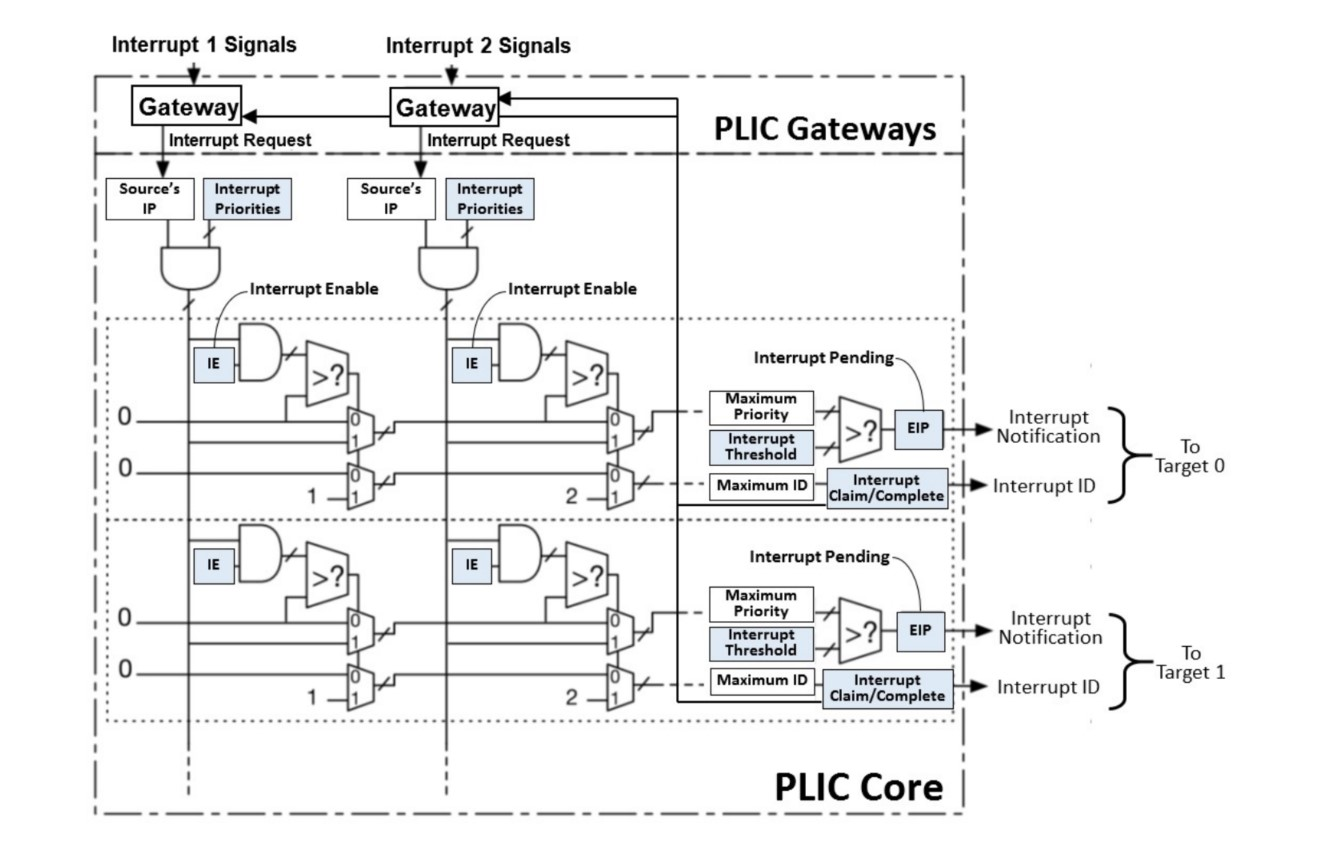
\includegraphics[width=1\textwidth]{thesis-images/PLIC.jpeg}
    \caption{PLIC 架构\cite{riscv-plic}}\label{fig:PLIC}
\end{figure}

在介绍如何模拟 PLIC 来进行中断注入前首先需要介绍一下 RISC-V PLIC 的结构。PLIC 是由 sifive 首先提出的一种基于 RISC-V 的中断控制器,用于处理来自外部设备的中断请求。PLIC 是一个通用的可扩展中断控制器,可以在系统上处理大量的中断请求。它可以与多个处理器核心链接,允许这些核心同时响应不同的中断请求。它的设计具有高可扩展性,可用于不同大小和复杂度的处理器系统。

图~\ref{fig:PLIC}~展示了 PLIC 的架构图,PLIC 可以转发单个中断源到到多个 CPU 核心。在进入 PLIC 处理函数后,CPU 将会读取 claim 寄存器获取中断号。成功读取后 PLIC 将会自动清除 PLIC pending 寄存器中的 pending 位,宣称这个中断已经被服务。除此之外,若 pending 位没有被设置时去读取 claim 寄存器也是合法的。举例来说,当一个全局中断被路由到多个 CPU,同时一个 CPU 已经在另一个 CPU 读取 claim 寄存器前读取了这个寄存器,上述的情况将会发生。

\begin{figure}[]
    \centering
    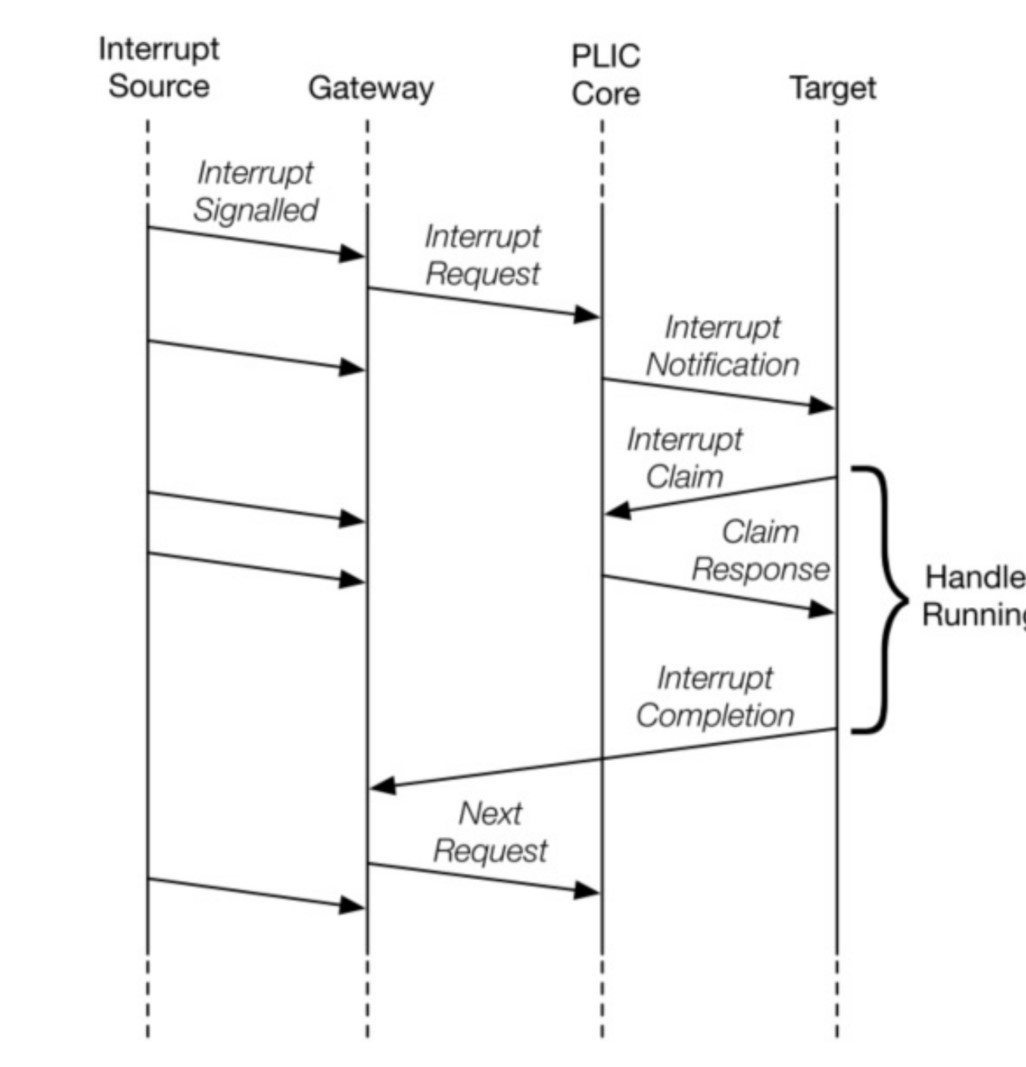
\includegraphics[width=1\textwidth]{thesis-images/irq-flow.jpg}
    \caption{PLIC 中断处理流\cite{riscv-plic}}\label{fig:irq-flow}
\end{figure}

图~\ref{fig:irq-flow}~展示了 PLIC 的中断流程,具体描述如下:
\begin{enumerate}
    \item 全局中断从中断源送到中断网关。
    \item 中断网关向 PLIC core 发送单个中断请求,PLIC core 将中断请求存放在 pending bits 中。
    \item 检查是否对于中断优先级设置了阈值,如果中断优先级超过了阈值,则将中断发送给一个或多个 CPU core。
    \item CPU core 接收到外部中断时,它会发送中断声明请求去获取 PLIC core 为该中断存储的最高优先级的全局中断标志符。
    \item PLIC core 清除相应的中断 pending bit。
    \item CPU core 处理中断后告知 PLIC,PLIC 向对应的中断网关发送中断完成消息。
    \item 中断网关现在可以转发相同中断源的中断请求给 PLIC core。
\end{enumerate}

因此,要模拟 PLIC 并实现中断投递,至少要对以下几个方面进行实现:
\begin{enumerate}
    \item 对于 PLIC 的 MMIO 寄存器进行模拟。
    \item 拦截读写 PLIC MMIO 寄存器的并进行模拟,虚拟机监控器需要维护一套 PLIC 结构并模拟读写过程。
    \item 中断首先发送到虚拟机监控器,虚拟机监控器根据 hart 上下文向 PLIC 读取中断号并存储中断号且设置中断等待,随后向客户操作系统转发。
    \item 客户操作系统完成中断处理后,向 complete 寄存器写入表明完成,虚拟机监控器拦截并向 PLIC 发送完成请求并将 pending 位清零。
\end{enumerate}

\begin{table}[htbp]
    \caption{PLIC 模拟结构体}\label{tab:table4}
    \vspace{0.5em}\centering\wuhao
    \begin{tabular}{p{5cm}p{5cm}p{5cm}}
    \toprule[1.5pt]
    成员变量&类型&描述\\
    \midrule[1pt]
    field&类型&描述\\
    base&u64&PLIC 基地址\\
    source\_priority&[u32; 512]&中断源优先级\\
    pending&[u32; 16]&中断等待位\\
    enable&[[u32; 32]; MAX\_CONTEXTS]&中断使能位\\
    thresholds&[u32; MAX\_CONTEXTS]&中断阈值\\
    claim\_complete&[u32; MAX\_CONTEXTX]&中断宣称/完成位\\
    \bottomrule[1.5pt]
    \end{tabular}
    \vspace{\baselineskip}
    \end{table}

表~\ref{tab:table4}~展示了虚拟机监控器在实现过程中为 PLIC 模拟的 MMIO 寄存器及实现类型的描述。

文章在之前提到,hypocaust 与 hypocaust-2 在实现方面有一些不同,这是由于在开启了 RISC-V Hypervisor Extension 的状态下,硬件会提供一个名为 hvip 的寄存器用来标志 VS-mode 的中断,因此只要对 hvip 对应的标志位进行标记,当特权级返回 VS-mode 的时候硬件会自动陷入中断处理流程。而 hypocaust 则需要完全软件模拟硬件的流程,即:
\begin{itemize}
    \item 设置 sip 寄存器,表示发生中断。
    \item 设置 scause 寄存器,表示陷入原因。
    \item 设置 sepc 寄存器,重定向到客户操作系统的中断处理流程。
    \item 设置 sstatus 寄存器,表示当前处于 S-mode。
    \item 将 stval 寄存器清零。
\end{itemize}

\section{小结}

本章详细地介绍了 hypocaust 与 hypocaust-2 两版虚拟机监控器的实现方法,对于 CPU 虚拟化、内存虚拟化、I/O 虚拟化 
以及中断虚拟化等虚拟机监控器所需要的主要功能进行了详细的介绍,同时为了便于读者理解,也穿插了一些对于 RISC-V 体系结构和
Rust 编程语言的介绍。



\chapter{系统实现结果}
由于目前市面上仍没有实现了 RISC-V Hypervisor Extension 的流片,因此本课题一直使用 QEMU 7.1.0 用于模拟硬件,QEMU 在 7.0.0 版本后就默认提供了 RISC-V Hypervisor Extension。QEMU 在启动后进行一系列初始化操作后跳转到 0x80000000(RAM 起始地址)开始执行 RustSBI,RustSBI 运行在 M mode,会对 CPU、内存、外设等进行一系列探测与初始化。例如对 UART、CLINT 做一些初始化工作,同时设置 PMP 寄存器以实现内存隔离。之后跳转到 0x80200000 开始执行第一条指令。

\section{hypocaust 启动并运行 minikernel}
minikernel 是由清华大学 rCore-Tutorial-v3 裁剪而来的最小的带文件系统的内核,是一个最简单的操作系统内核。此时内核中已经运行了文件系统,即已经使用了 virtio 等 I/O 功能,因此在虚拟机监控器中必须实现 I/O 虚拟化以及中断虚拟化。

同时,从运行 minikernel 开始此时所要运行的已经是一个完整的操作系统内核而不是简单的测试应用程序,因此则在虚拟机监控器的实现中引用了基于设备树配置的技术。

这里首先介绍一下什么是设备树,设备树(device tree)机制时 Linux 内核从 Linux-3.x 版本引进的一种机制,目的是解决内核源码中 arch 目录下代码混乱的问题,这是由于在 arch 目录下存放着几百个开发板相关的文件,内核与这些硬件耦合,会导致内核代码混乱不堪。因此引入了设备树机制用来描述板级信息。

回到正文,本课题共使用了两种设备树机制,一种是用来配置运行在虚拟机监控器下的物理硬件的信息,用来初始化 hypervisor 的信息;另一种设备树是描述客户操作系统的设备树信息,用于 hypervisor 初始化客户操作系统并用于恒等映射。
\begin{figure}[]
    \centering
    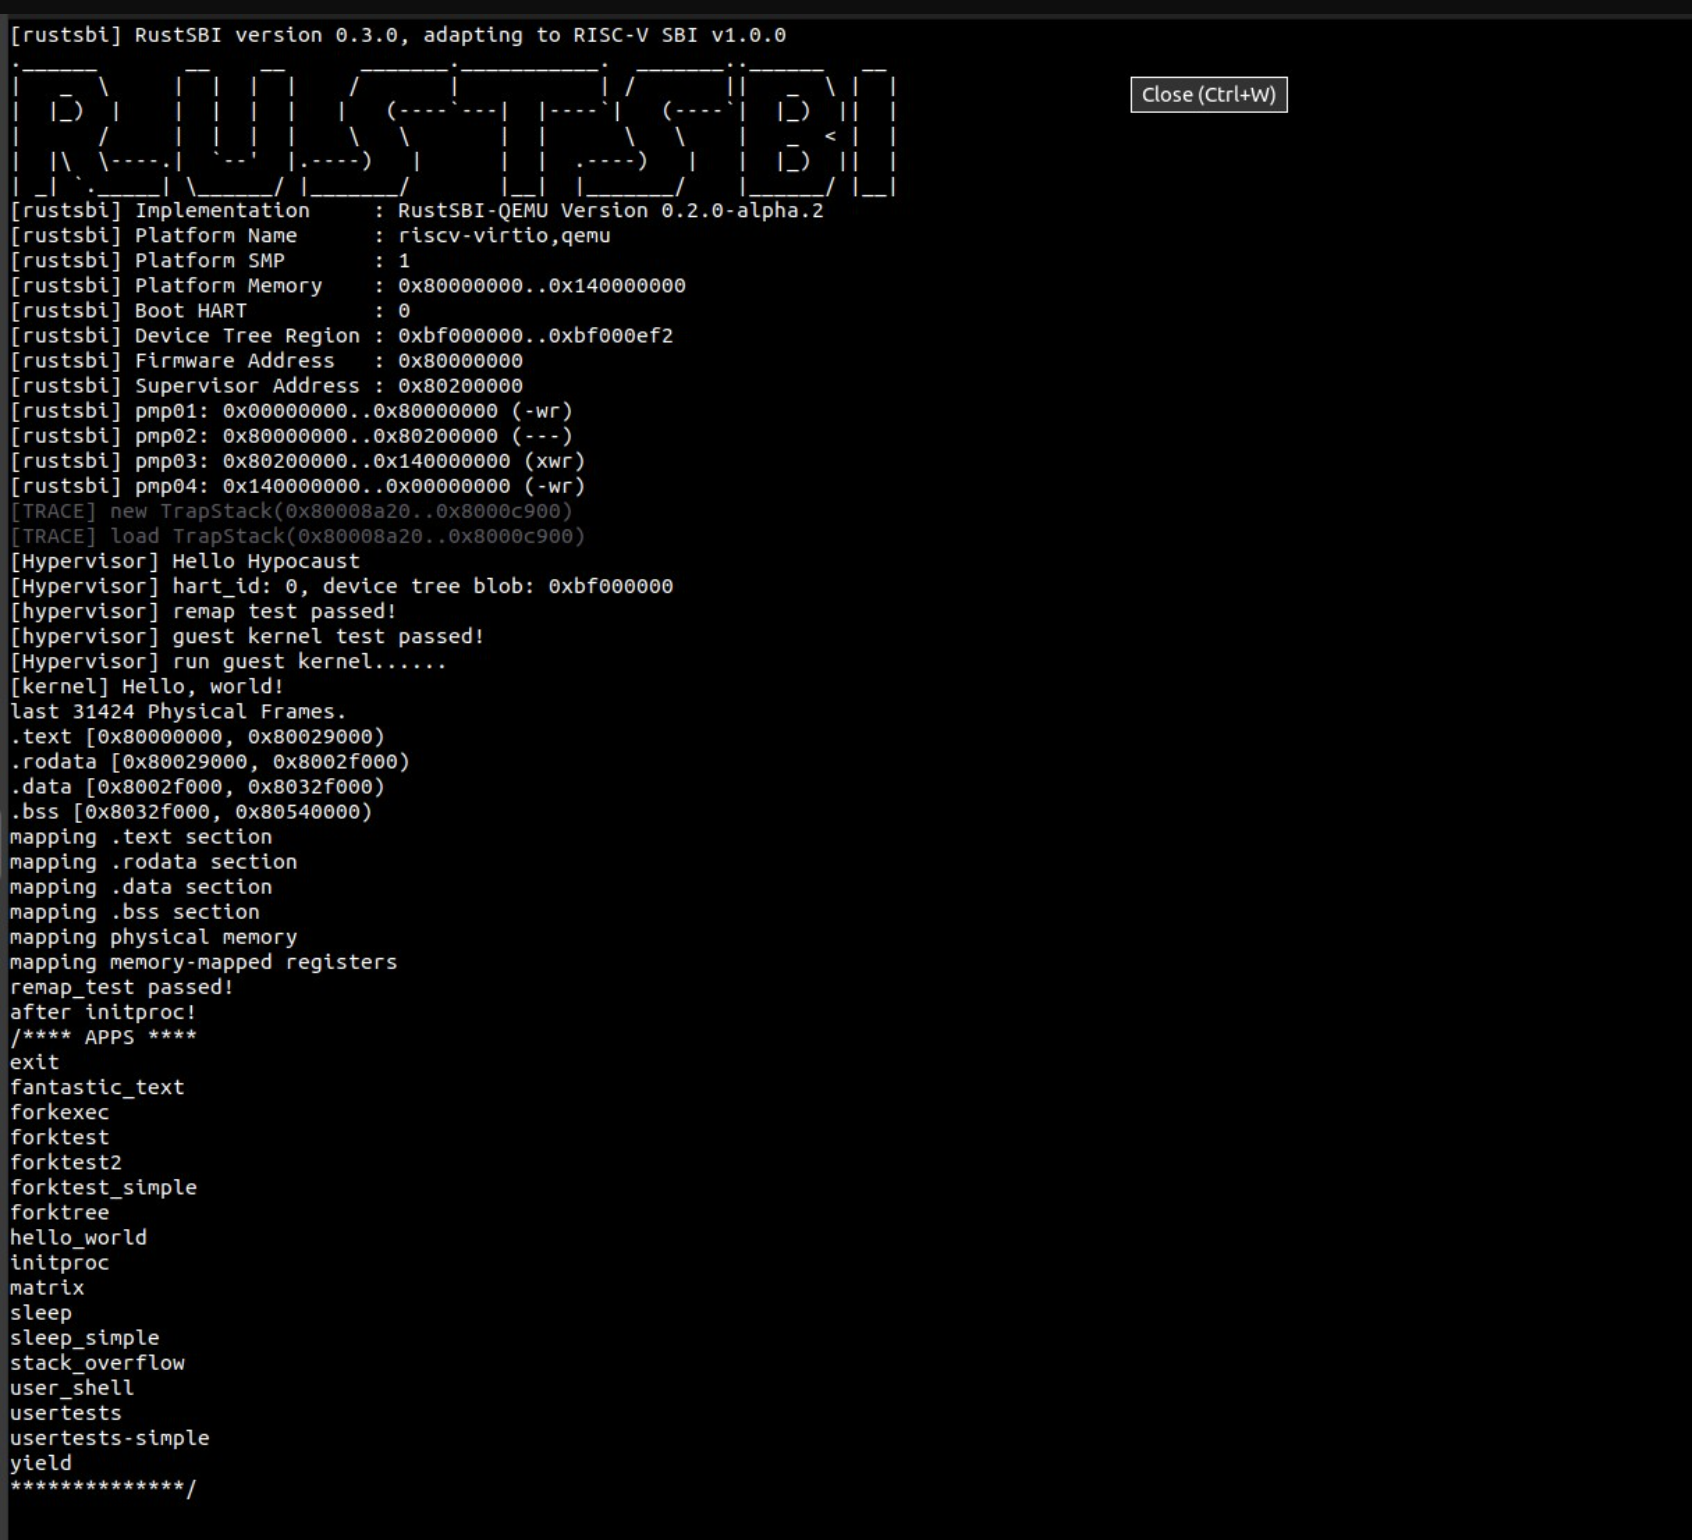
\includegraphics[width=0.6\textwidth]{thesis-images/hypocaust-run1.png}
    \caption{hypocaust 启动 minikernel 并进入 shell}\label{fig:hypocaust-run1}
\end{figure}

图~\ref{fig:hypocaust-run1}~展示了 hypocaust 启动并进入 shell 的运行结果截图。hypocaust 首先解析设备树并进行初始化,随后加载客户操作系统 ELF 并进行地址映射,最终跳转到客户操作系统并运行。

\begin{figure}[]
    \centering
    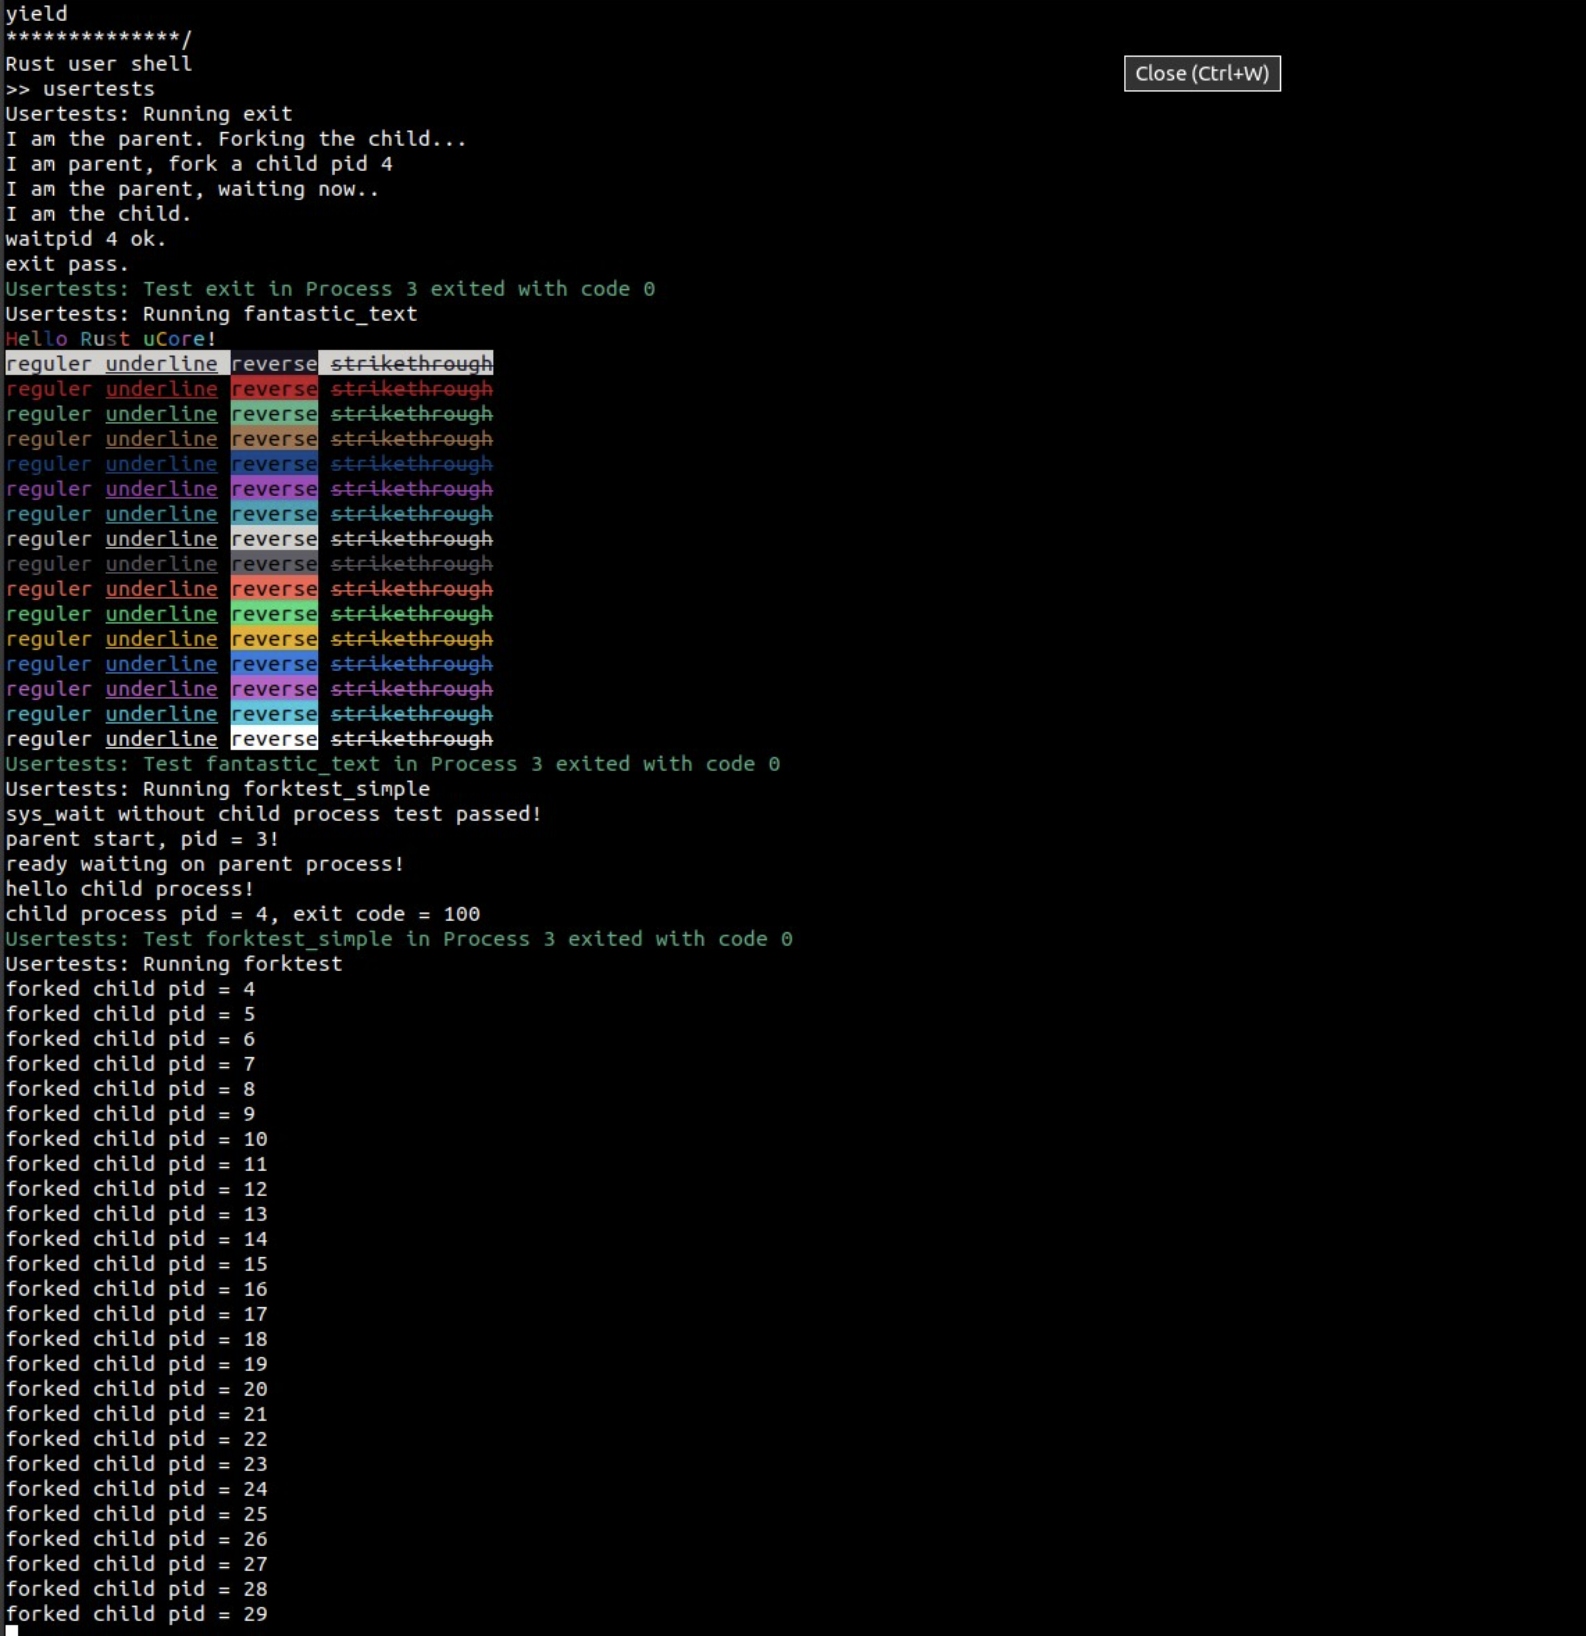
\includegraphics[width=0.6\textwidth]{thesis-images/hypocaust-run-2.png}
    \caption{hypocaust 运行用户态测试用例}\label{fig:hypocaust-run2}
\end{figure}

图~\ref{fig:hypocaust-run2}~展示了 hypocaust 启动的 minikernel 运行用户测试用例。

\section{hypocaust-2 启动并运行 rCore-Tutorial-v3}
rCore-Tutorial-v3 相较于 minikernel 增加了其他 I/O 设备以及增加了条件变量,因此对于虚拟机监控器来说并没有需要太多需要迭代的部分,因此在成功运行 minikernel 后再运行 rCore-Tutorial-v3 并没有遇到什么困难。

图~\ref{fig:hypocaust-2-rCore-Tutorial-v3-1}~与 图~\ref{fig:hypocaust-2-rCore-Tutorial-v3-2}~展示了 hypocaust-2 启动并运行 rCore-Tutorial-v3 的运行结果截图。



\begin{figure}[]
    \centering
    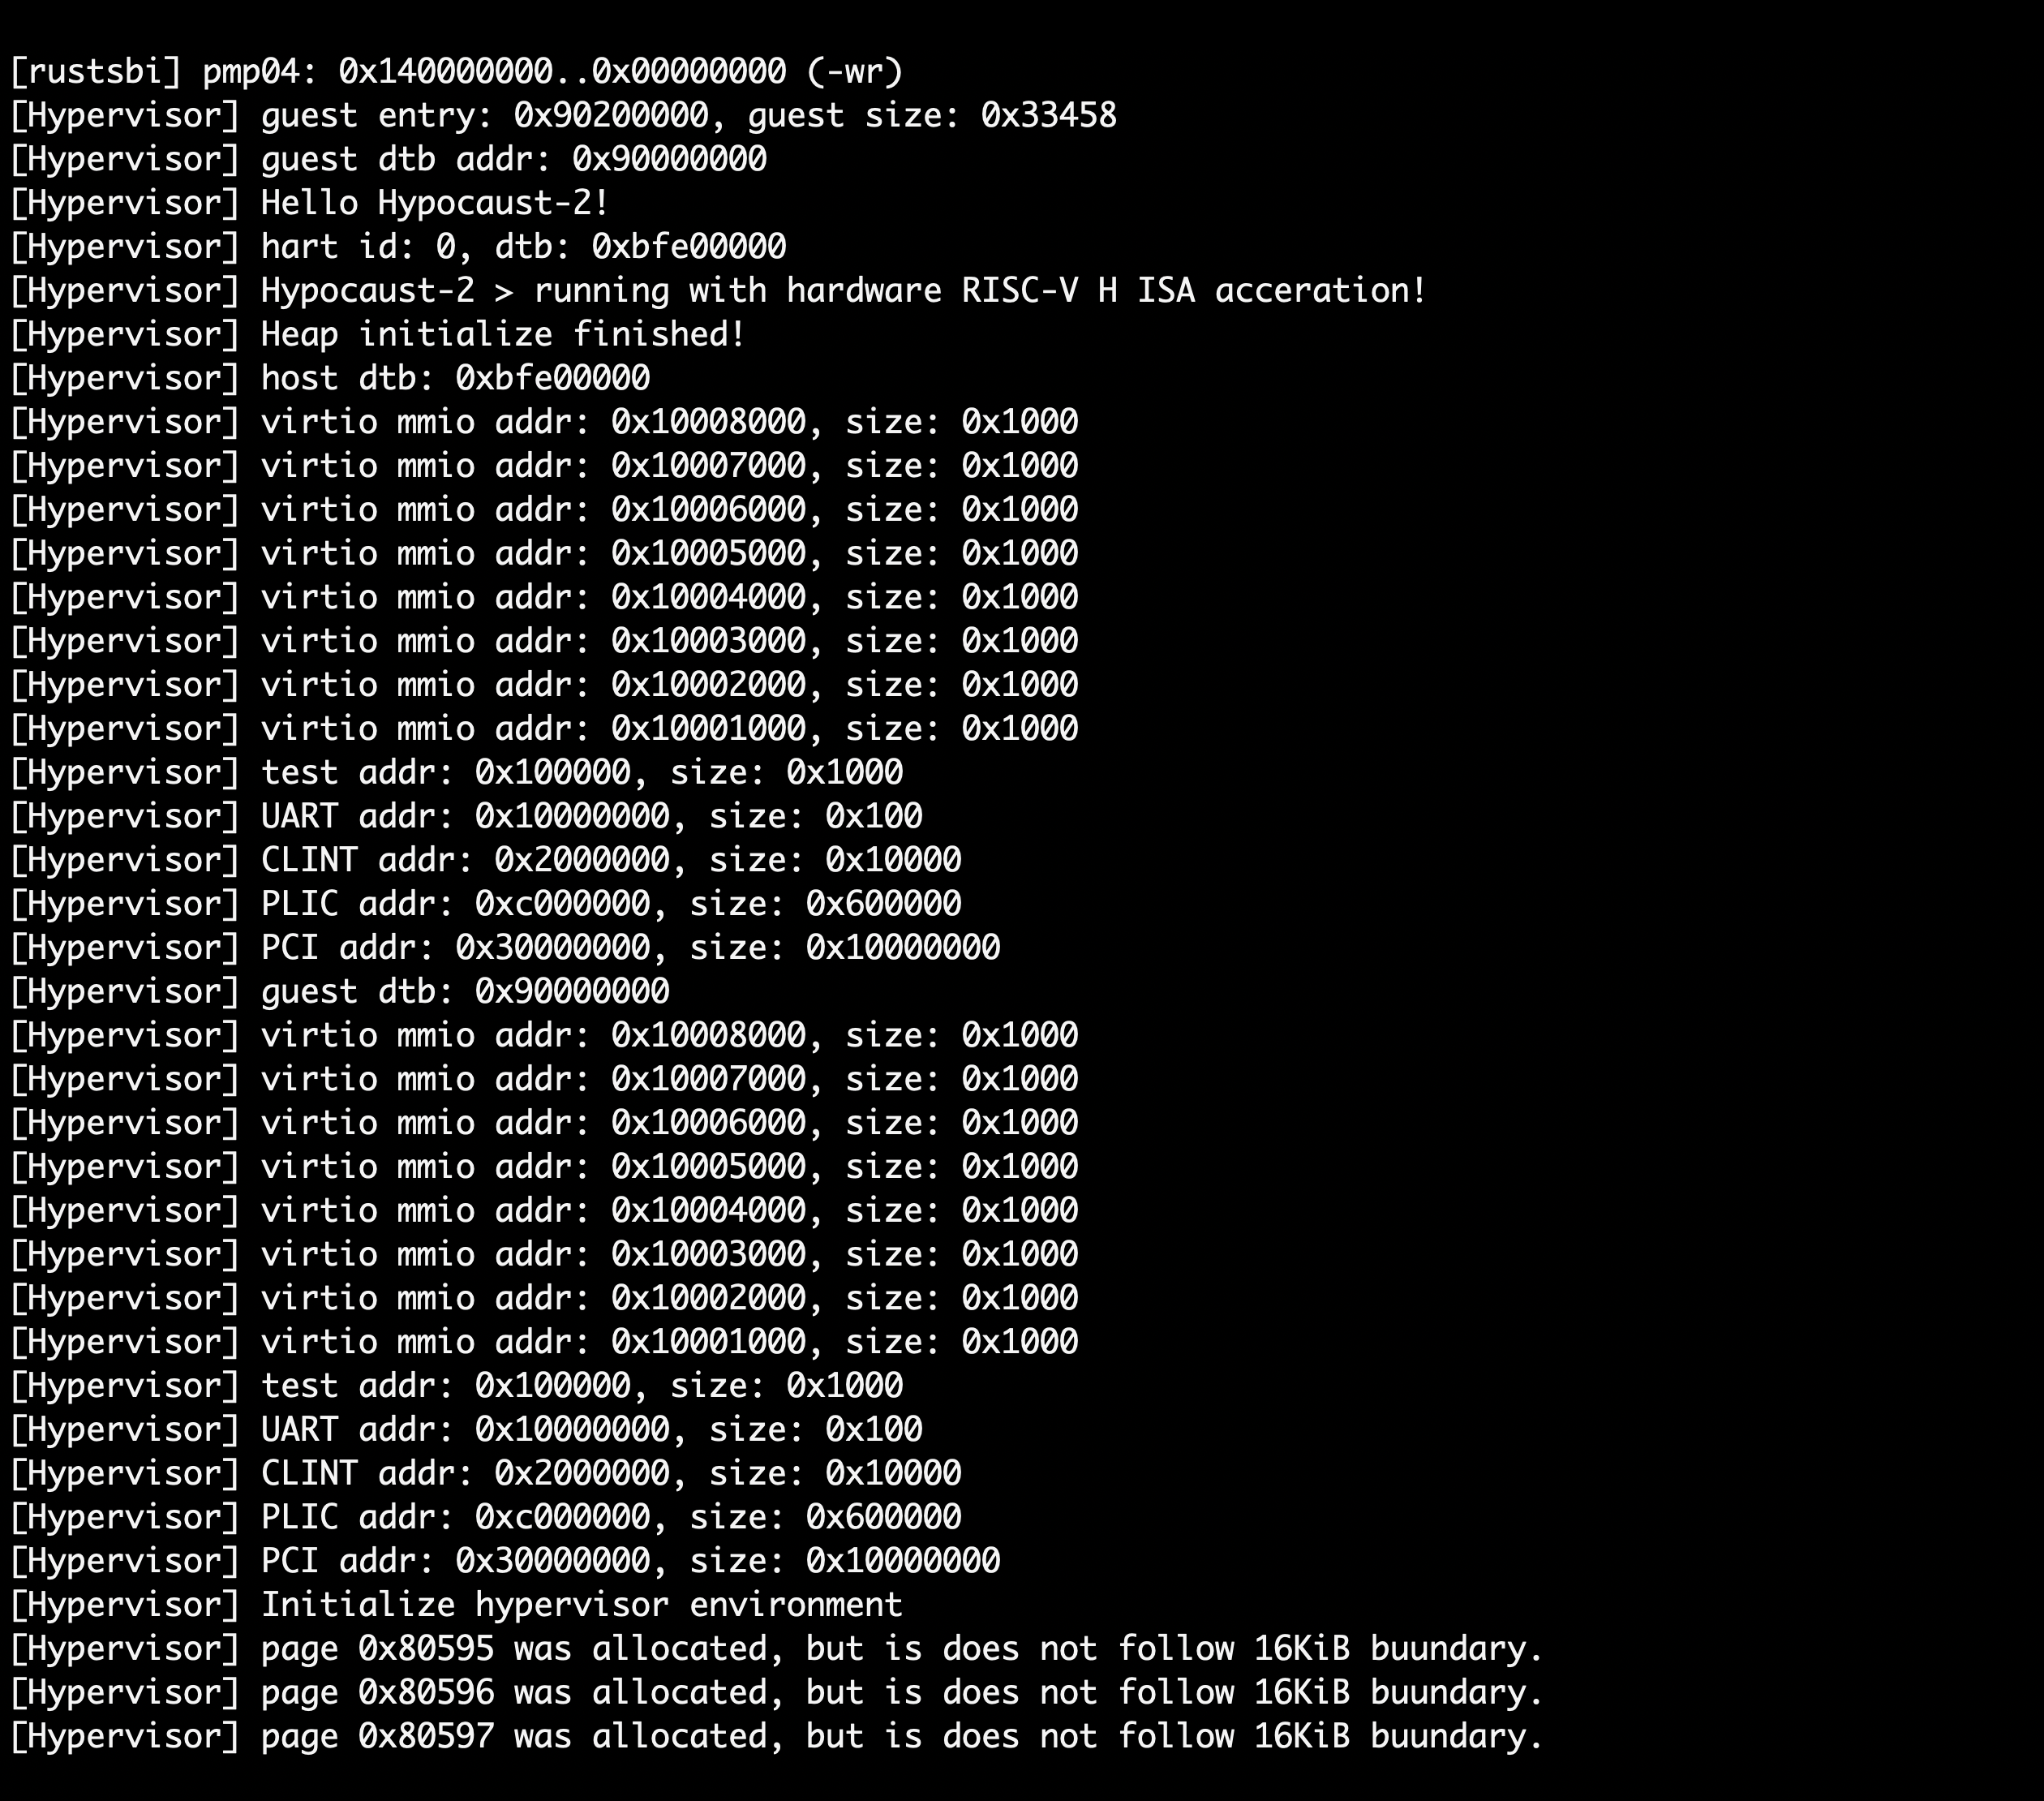
\includegraphics[width=0.6\textwidth]{thesis-images/hypocaust-2-rCore-Tutorial-v3-1.png}
    \caption{hypocaust 启动 rCore-Tutorial-v3}\label{fig:hypocaust-2-rCore-Tutorial-v3-1}
\end{figure}

\begin{figure}[]
    \centering
    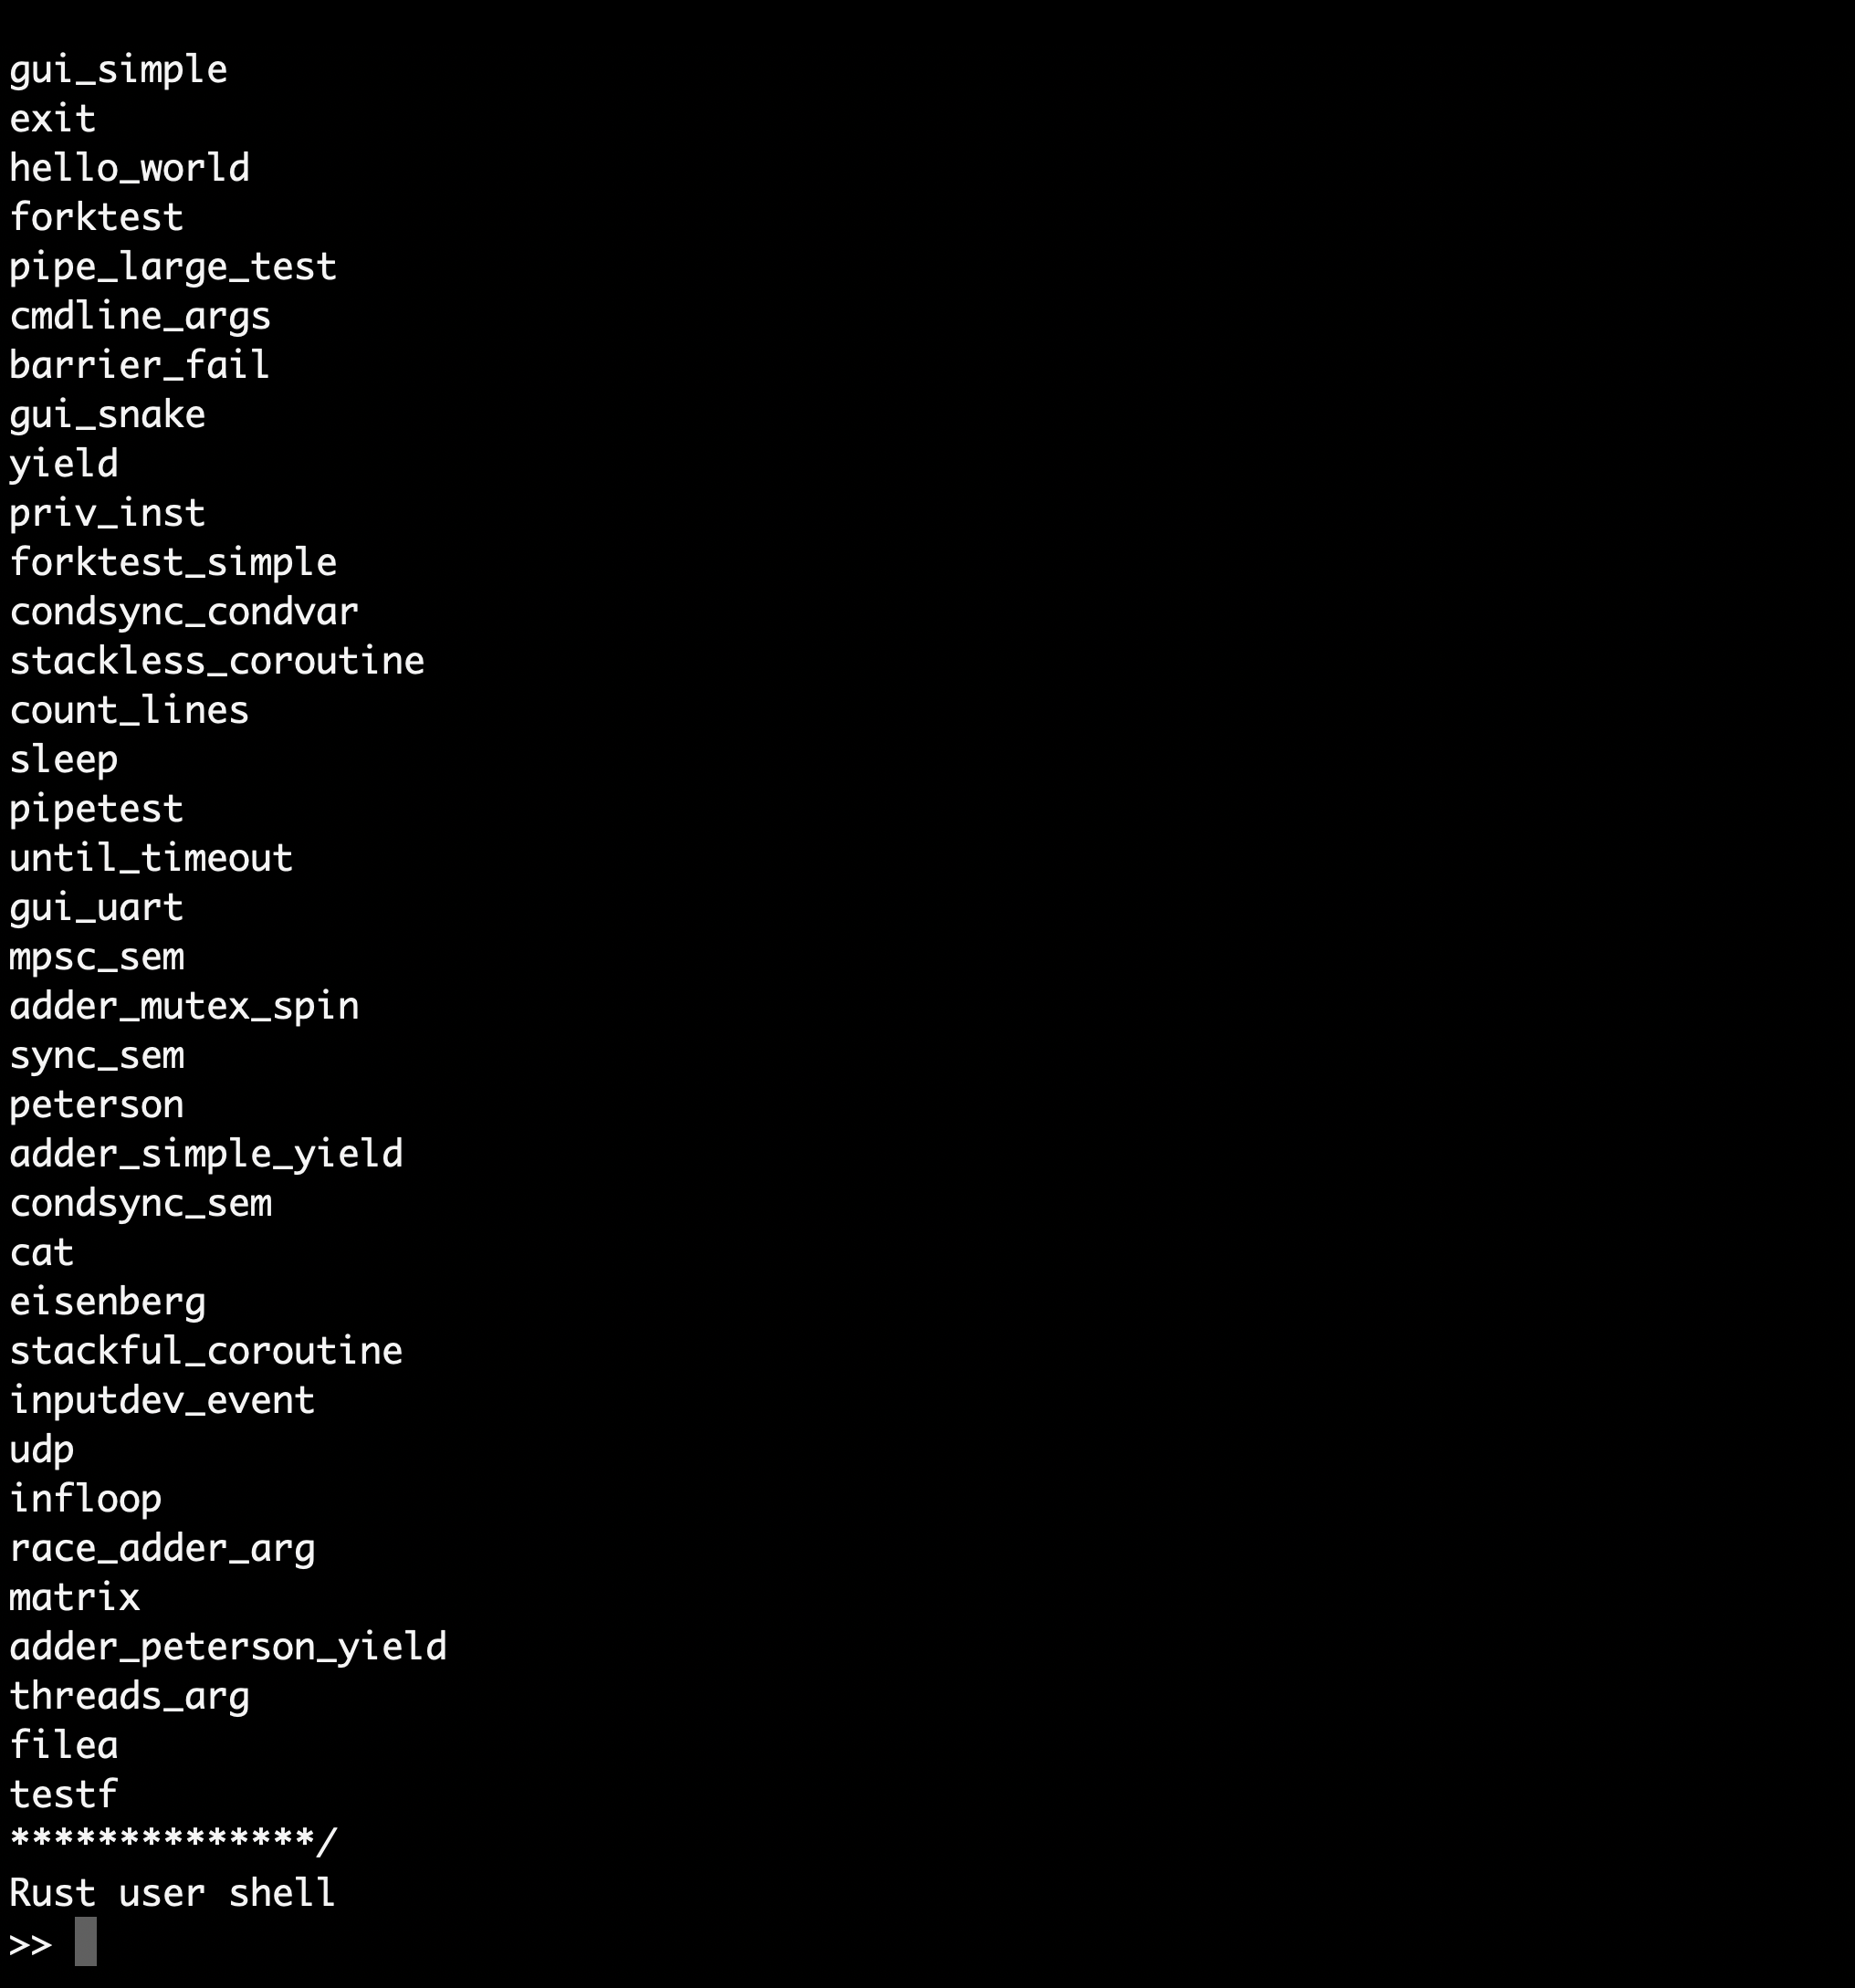
\includegraphics[width=0.6\textwidth]{thesis-images/hypocaust-2-rCore-Tutorial-v3-2.png}
    \caption{hypocaust 进入 rCore-Tutorial-v3 shell}\label{fig:hypocaust-2-rCore-Tutorial-v3-2}
\end{figure}

\section{hypocaust-2 启动并运行 RT-Thread}
RT-Thread 是一个开源的 IOT 实时操作系统,RT-Thread 是本项目运行的第一个运行的工业级别的操作系统。RT-Thread 给了很详细的文档,在阅读完文档后成功编译了一个可以运行在 qemu-system-riscv64 的 RT-Thread 版本,在添加了部分 sbi call 的处理后成功启动并运行了 RT-Thread。

图~\ref{fig:hypocaust-2-rt-thread}~展示了 hypocaust-2 启动并运行 RT-Thread 的结果截图。

\begin{figure}[]
    \centering
    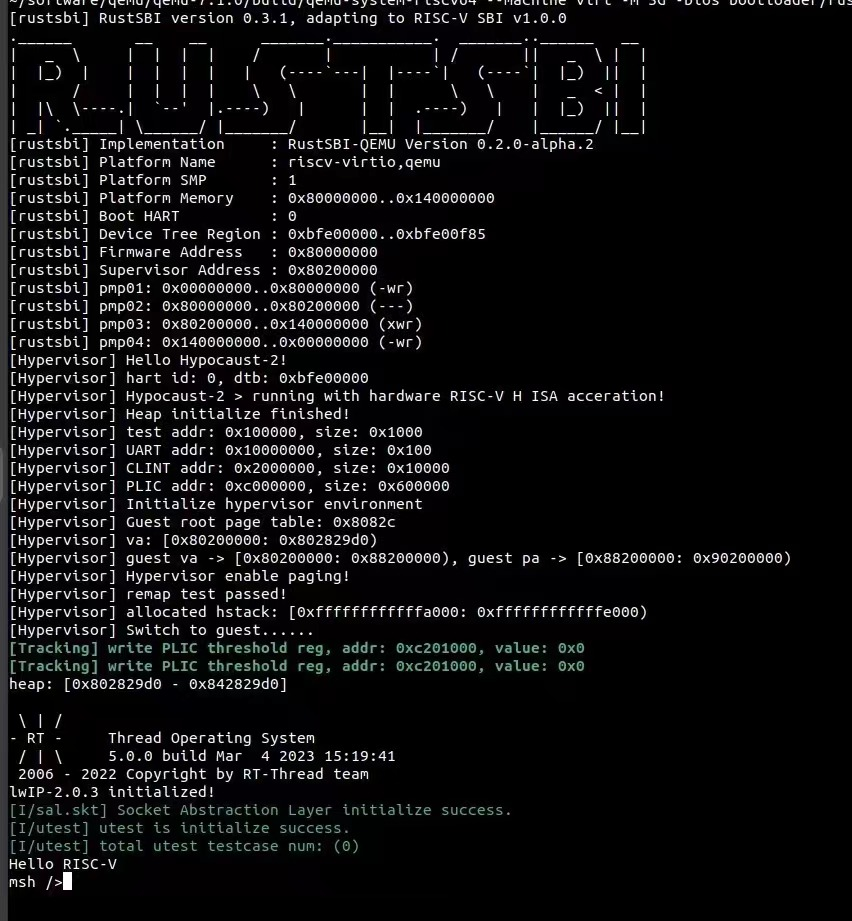
\includegraphics[width=0.6\textwidth]{thesis-images/hypocaust-2-rt-thread.jpeg}
    \caption{hypocaust 启动并运行 RT-Thread}\label{fig:hypocaust-2-rt-thread}
\end{figure}


\section{hypocaust-2 启动并运行 Linux mainline}
Linux 是当前世界上最重量级的开源的通用操作系统,因此能够在自己构建的系统中成功跑起 Linux 是每一位做体系结构或者做系统人的目标。本课题成功在 hypocaust-2 上运行了主线 Linux 并进入了 shell 执行命令,在调试的过程中也遇到了一些坑,下面将尝试说明在运行 Linux 过程中遇到的问题及解决方法:
\begin{enumerate}
    \item 首先根据运行 Linux 过程中触发的未实现的 sbi call,并对其进行实现。
    \item 由于 hypocaust-2 只实现了 Sv39 级别的页表机制,而 Linux 采取了页表跌落方法来设置页表机制,即从 Sv57 开始探测,若 Sv57 映射失败,则向下尝试 Sv48,Sv39。由于只实现了 Sv39 机制,因此若发生了页表错误,虚拟机监控器需要手动进行两阶段页表翻译并得到主机物理地址,这样会造成错误。因此在经过一番探索后,给 Linux kernel 打了个 patch,强制使用 Sv39 页表(后来发现也可以给 qemu 打 patch 使其不支持 Sv48 和 Sv57)。
    \item 继续尝试运行 Linux kernel,发生了 softlock 问题,所谓 softlock 的意思就是一直停留在同一个进程而长时间不进行切换。在一番探索后发现是由于对于页表地址的处理有一些问题,对于一些未处理的地址直接跳过而没有进行 panic。
    \item 继续运行 Linux kernel,发生了一个 unhandled signal 4 code 0x1,该错误是在执行 \_\_fstate\_restore 第一条指令发生了错误,这是由于当前并没有开启浮点指令,因此需要重新编译 riscv64-gnu-toolchain,在编译时需要添加 --witch-arch=rv64imac --witch-abi=lp64 来编译不带浮点数的工具链。最终使用重新编译的工具链再次编译 busybox 和 Linux kernel 即可成功运行。
\end{enumerate}

图~\ref{fig:hypocaust-2-linux}~展示了 hypocaust-2 启动并运行主线 Linux 的结果截图。

\begin{figure}[]
    \centering
    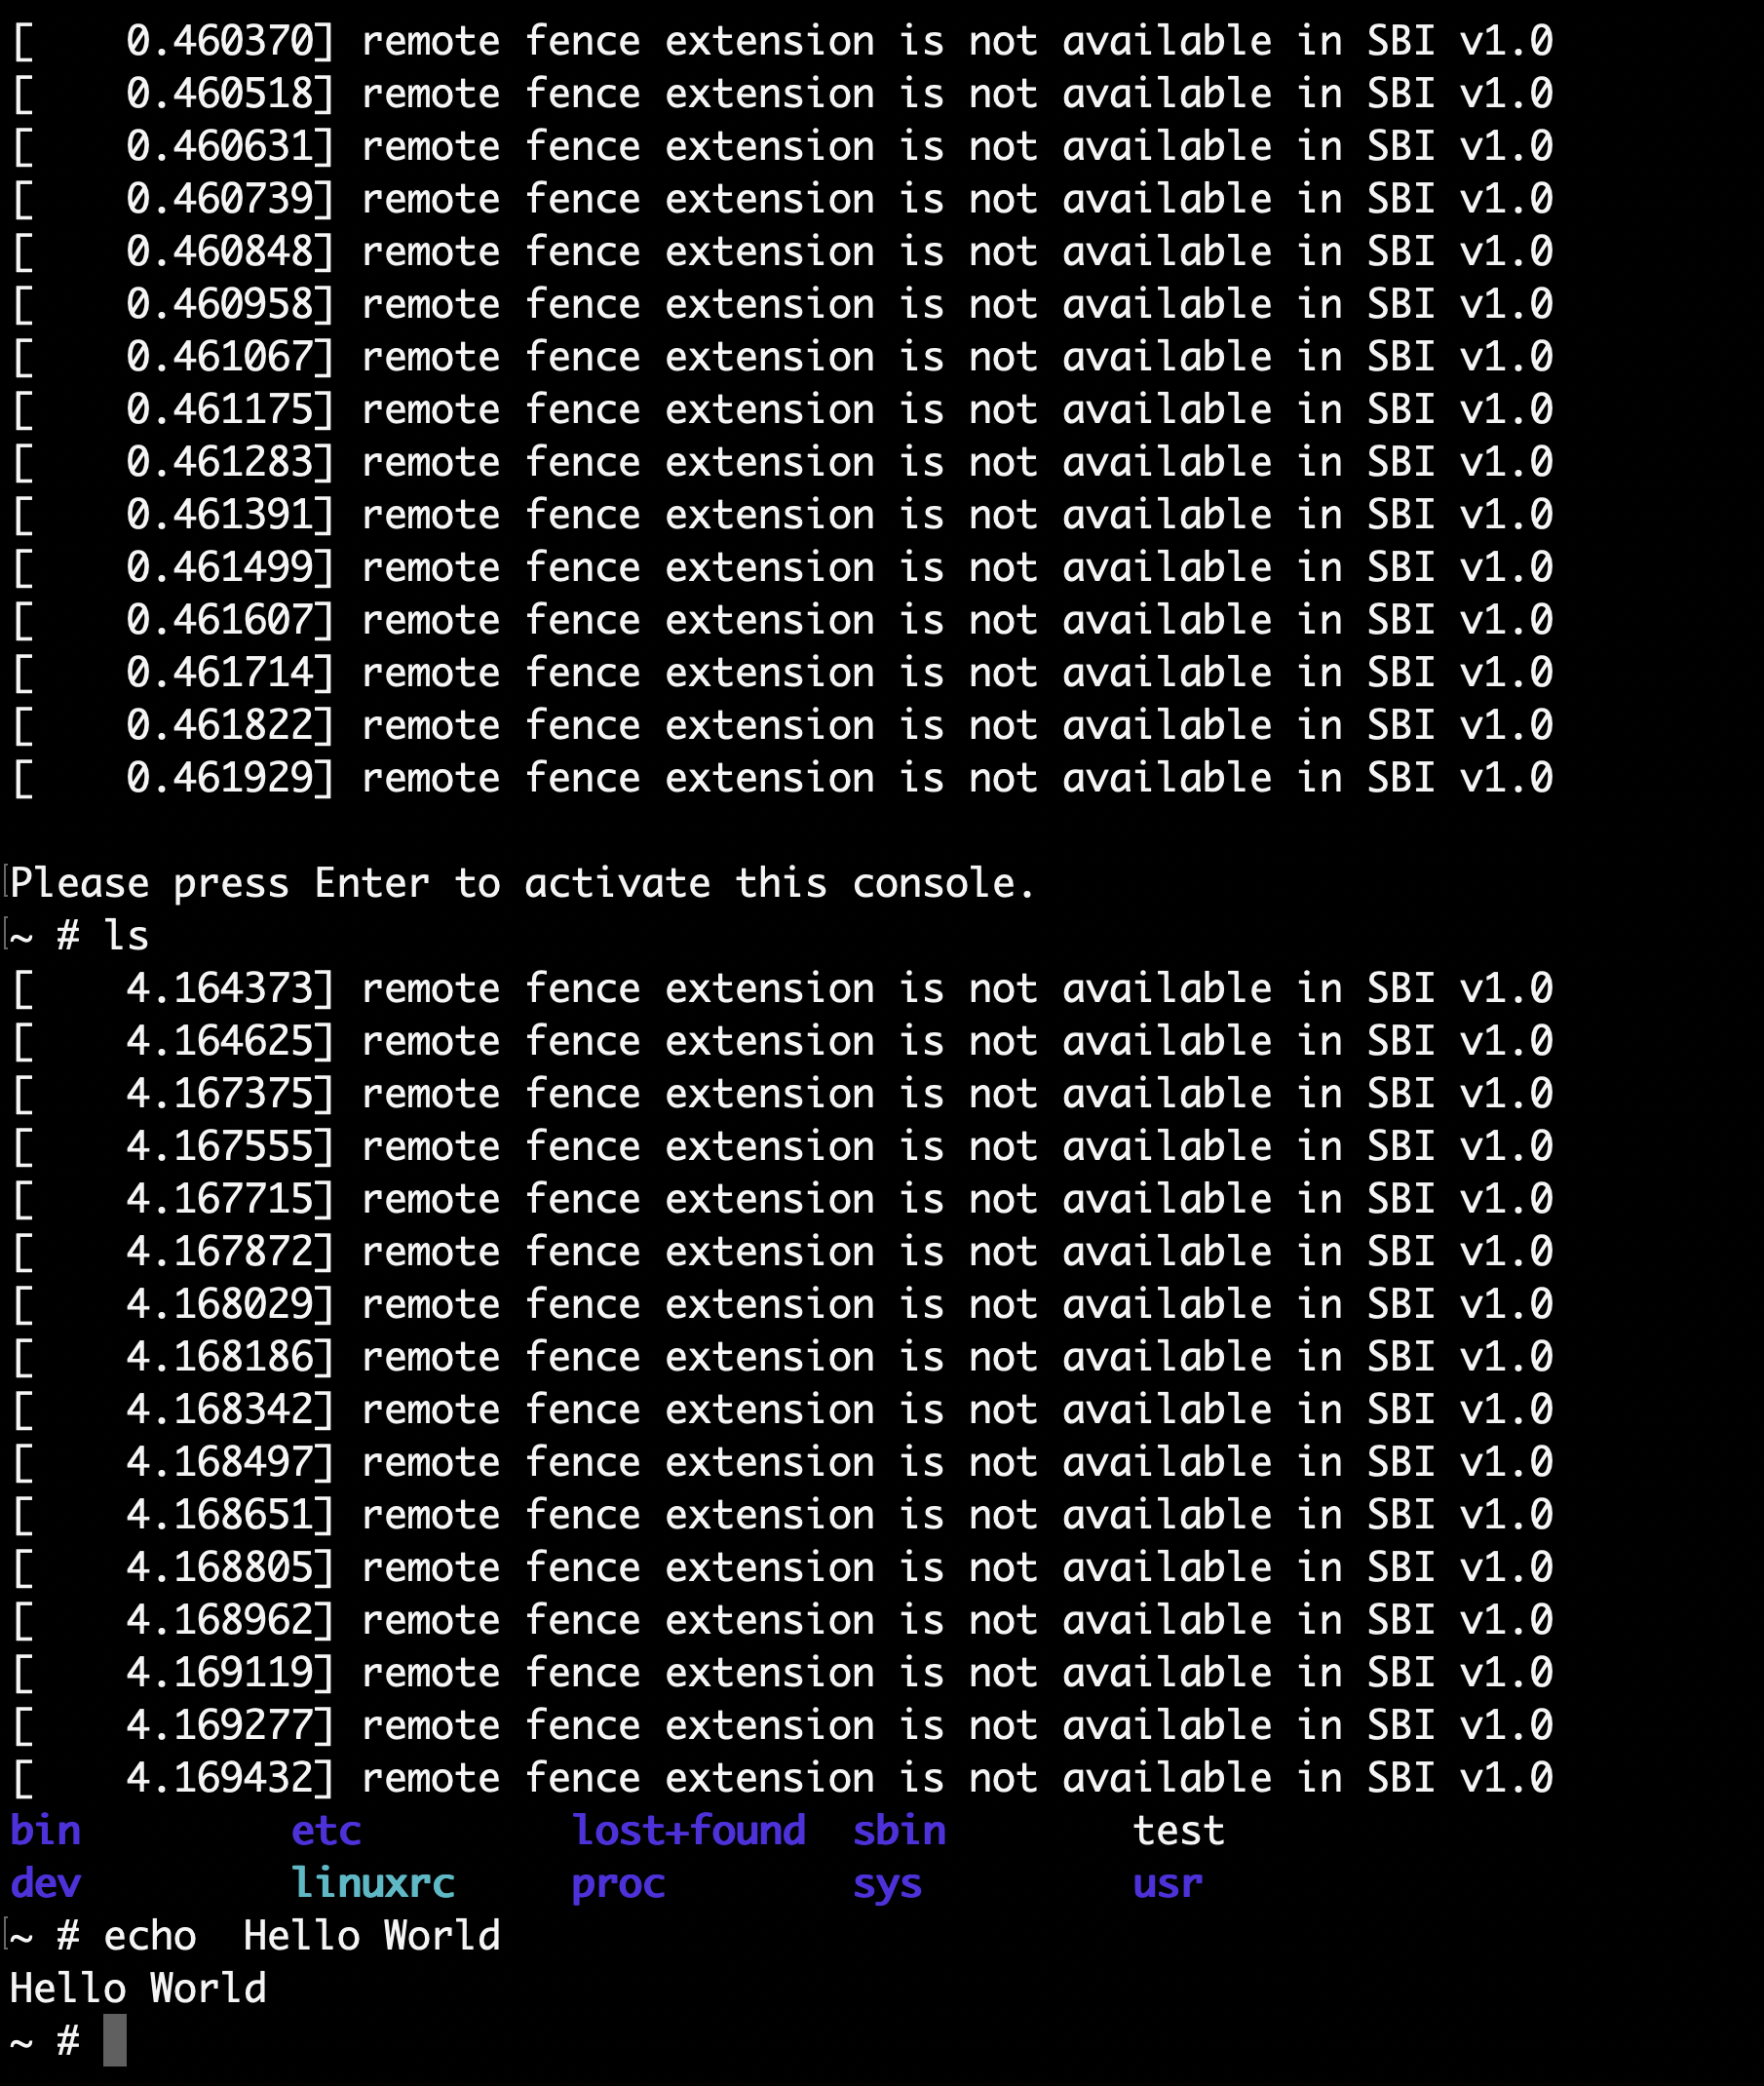
\includegraphics[width=0.75\textwidth]{thesis-images/hypocaust-2-linux.png}
    \caption{hypocaust 启动并运行主线 Linux}\label{fig:hypocaust-2-linux}
\end{figure}

\section{Benchmark}
本课题还尝试为项目添加 benchmark 以测试性能,并且创建了一个名为 hyperbench-riscv-rs 的项目,在该项目中参考了 \textbf{Hyperbench} \cite{wei2019hyperbench} 的实现,分别为 CPU 虚拟化、内存虚拟化、I/O 虚拟化分别写了测试用例,并考虑到了 idle 为 benchmark 带来的额外的开销。但最终后测试结果并没有办法得到预期的精确结果,理由是 qemu 并非是一个周期精确性模拟器,对于 TLB miss 等行为也无法精确模拟,因此无法作为一个可靠的性能测试结果,例如,在 QEMU 上同时运行内存热访问与冷访问时得到的结果是差不多的。

尽管在这里编写的 micro benchmark 并不能在 QEMU 上精确地测试出性能,但是仍然可以粗略地估计 hypocaust-2 与 RVirt 的性能差异。同样是启动 Linux,hypocaust-2 可以在几秒内启动 Linux,而 RVirt 则需要在几分钟内才可以启动 Linux,因此,相较于 RVirt,hypocaust-2 具有极大的性能优势。
因此,在本节中将尝试简要分析 hypocaust-2 与 RVirt 实现的异同,并分析本课题的成果的优势与不足。

\subsection{Rvirt 与 hypocaust-2 的实现比较}

相比于 hypocaust-2 的硬件虚拟化,与 hypocaust 类似,RVirt 采用的是纯软件虚拟化技术。RVirt 既可以基于 RISC-V Berkeley bootloader 启动也可以基于
RVirt 自己实现的 bootloadr 启动。在启动并进入 S mode 之后 Rvirt 首先获得客户操作系统的设备树信息,随后根据设备树信息初始化设备以及构建影子页表并加载客户操作系统,RVirt 中所有数据结构
全部被存储在一个名为 \textbf{Context} 的结构体中。除此之外,RVirt 也维护了一个名为 \textbf{Shared} 的结构体,用于存储多核之间的共享数据,
包括 \textbf{boot\_page\_table(启动页表)}、\textbf{ipi\_reason\_array(核间通信信息)}、\textbf{uart\_writer(共享互斥的 UART)} 以及 \textbf{hart\_lottery(用于在多个 hart 之间进行公平工作的 AtomicBool 类型)}。

在 RVirt 初始化后将向其他核发送 IPI 请求(如果有的话),随后将核信息存储到 ipi\_reason\_array 中并切换上下文进入客户操作系统入口进行执行。由于没有启用硬件虚拟化的支持,因此 RVirt 不得不依赖于 RISC-V 原有的特权级进行隔离,
客户操作系统运行在 U mode,当执行到特权指令时将会陷入到 Rvirt 中,Rvirt 将首先保存上下文并执行 \textbf{strap} 进行陷入处理,随后恢复上下文并返回客户操作系统继续执行。
hypocaust-2 与之相比,由于 hypocaust-2 硬件中维护了一套 vs 开头的寄存器并添加了 VS mode 来进行隔离,因此 hypocaust-2 无需对每个陷入的特权指令进行处理(同时也可以配置哪些特权指令需要陷入虚拟机监控器进行处理)。
因此在 hypocasut-2 的性能在这方面要比 RVirt 高出很多。

从内存虚拟化的角度说,RVirt 使用了影子页表技术进行维护,在之前的章节中已经对于影子页表技术进行了简要的介绍,这里不再进行赘述,本段主要描述 RVirt 的内存虚拟化的具体实现。
Rvirt 为客户操作系统维护了一个 \textbf{PageTables} 的数据结构,在 PageTabls 中维护了一个大小为 4,类型为 u64 的数组,分别表示 UVA(用户虚拟地址)、KVA(内核虚拟地址)、MVA(机器虚拟地址)以及 MPA(机器物理地址)。
当 RVirt 启动时,首先会根据设备树分别映射 Host 以及 Guest 的内存地址,并将其放在 MPA 页表根地址中并进行页表安装,随后进入 Guest 执行。当客户操作系统写入 \textbf{satp} 寄存器或执行 sfence.vma 命令时会陷入到 Rvirt 中,
Rvirt 会修改影子页表的映射并根据模拟的 sstatus 寄存器的值确定当前根页表所处的状态并进行重新安装页表。而 hypocasut-2 则使用了两阶段页表翻译技术,在第二阶段页表翻译使用了 Nested MMU,因此当客户操作系统修改页表时,实际上只修改了
第一阶段页表映射,在硬件层面实际上会进行两次页表遍历,因此当 guest 修改页表以及刷新页表时不需要陷入内核,极大地提升了性能。

从中断虚拟化的角度说,主要分为两个部分,即时钟中断和外部中断。时钟中断的处理相对简单,当 RVirt 收到时钟中断请求时,它将会查看当前时间戳是否大于模拟的 mtimecmp 寄存器。若小于,则直接屏蔽本次中断;若大于,则通过修改模拟的 sip 寄存器来注入中断,随后修改 sepc 寄存器 
到中断向量地址并进行中断的模拟。外部中断的处理则略显复杂。在 RVirt 中使用 PLIC 进行全局中断的转发与处理,在 Context 结构中维护了一个 irq\_map 的数据结构,用于将 host 外部中断号映射到 guest 外部中断号,当检测到外部中断时,RVirt 根据 host 外部中断号获取到 guest 外部中断号,
并根据 guest 中断号从模拟的 VirtIO 中得到对应的设备号,并查看是否被映射,若被映射则转发中断(与时钟中断的转发相同),若没有被映射则直接屏蔽中断。而 hypocaust-2 的处理则较为简单,当收到时钟中断时将 hvip 寄存器置位表示发生时钟中断,同时屏蔽时钟中断寄存器等待下次中断设置。当收到外部中断时,
根据模拟的 PLIC 中断号向 Guest 进行转发。尽管处理更加简单,但中断虚拟化的性能是相差不大的。

从 IO 虚拟化角度来说,RVirt 对于 VirtIO 进行模拟,它没有将 MMIO 空间暴露给 Guest,因此当 Guest 读写 MMIO 寄存器时需要陷入 RVirt,Rvirt 根据读写寄存器的值获得 Guest DMA 分配的客户虚拟地址,随后手动进行影子页表映射,将客户虚拟地址转化成主机物理地址并写入真实的 MMIO 寄存器,
当设备准备好数据后就会将准备好的数据放到对应 DMA 分配的帧中,随后 RVirt 得到外部中断并进行转发。而 hypocaust-2 则使用恒等映射进行设备透传,保证 DMA 分配的帧的客户虚拟地址和主机物理地址是相等的,因此不需要进行设备模拟与陷入,极大地提升了性能。

总结来看,hypocaust-2 在性能上比 RVirt 要强大得多,可以以近几十倍的速度启动 Linux,然而 hypocasut-2 在多核以及设备隔离上不如 RVirt 做得好,这也是之后本课题努力的方向。





\section{小结}

本章主要详细介绍了两版虚拟机监控器是如何一步步运行系统的,在本章中详细介绍了虚拟机监控器可以运行的系统,包括 minikernel、rCore-Tutorial、RT-Thread 以及 Linux kernel。
本章详细说明了本课题是如何使用迭代式开发与测试驱动开发一步步由简单到复杂运行起系统的,并对其中遇到的一些问题以及解决方法做了详细描述。

除此之外,本章也对 Benchmark 进行了一些尝试,同时对 RVirt 与 hypocaust-2 的设计与实现进行了比较和分析,并分析了其中的优势与不足,以便找到本课题后续发展的目标。

\chapter{总结与展望}

RISC-V 作为新兴的开源的指令集架构,在诞生之初就受到了全世界系统及体系结构开发者的关注。RISC-V 作为后起之秀,可以博采 x86、ARM 等指令集架构之众长,同时又不必受其兼容性之制约;同时 RISC-V 拥有一个受众广大且异常活跃的开源社区,开发者们纷纷在社区中提出自己的建设意见而后经过讨论得出最优的体系架构方案。而 RISC-V 虚拟化扩展正是由社区互相讨论与实践得到的结果。

本次课题从零到一实现了两版 RISC-V Type-1 hypervisor,并可以成功启动并运行 rCore-Tutorial-v3、RT-Thread、主线 Linux 等操作系统内核,本课题实现了国内首个使用 RISC-V 硬件辅助虚拟化技术实现的 RISC-V hypervisor,为国内该领域的研究填补上了一块空白,同时也为 RISC-V 虚拟化扩展开发提供了一条标准实现的路径。

本文首先对本课题研究的背景以及意义进行分析,随后对于目前存在的一些相关工作以及虚拟化相关的技术原理进行介绍。随后,本文详细介绍了课题实现的两个虚拟化软件,hypocaust 以及 hypocaust-2 的具体的设计与实现,并在最后给出了其运行各种系统的结果。

由于 RISC-V 虚拟化的生态仍不是特别完善以及时间原因,本课题仍有一些问题需要解决,下面给出接下来需要做的工作:
\begin{enumerate}
    \item 目前实现的 hypervisor 只能运行单核操作系统,下一步计划为操作系统提供多核支持,主要是通过添加核间通信以及同步原语来完成,最终可以运行多核操作系统并且可以同时运行多个操作系统。
    \item 目前实现的 hypervisor 只能支持单 guest,但是在实现过程中为之后实现多 guest 预留了实现空间。将在之后为 hypervisor 添加多 guest 调度算法以实现多 guest。
    \item 计划为 hypocaust-2 实现 AIA 以及 IOMMU 来提高中断虚拟化的性能以及保证 I/O 虚拟化的安全性和隔离型。
    \item 参考 unikraft\cite{kuenzer2021unikraft} 为 RISC-V hypervisor 封装为 OS 无关的硬件抽象库,在之后可以为 OS 所调用并可以很容易地创建 Type-1 或者 Type-2 hypervisor。
    \item 计划为 hypocaust-2 支持多个指令集架构,包括 x86、ARM 等,以实现多指令集架构的混合虚拟化。在之后也计划将其运行在实际的开发板上。
    \item 在体系结构层面对于虚拟机监控器进行优化,例如,可以通过减少 Page Walk 以及 TLB miss 次数\cite{park2022every, barr2010translation}、哈希页表\cite{yaniv2016hash} 等方式对性能进行优化。
    \item 本课题目前只做了部分 micro benchmark,计划在之后进行更多 micro benchmark 与 real world benchmark。
\end{enumerate}



